
\chapter{Docking Success Probability Prediction based on Stochastic Approximation}

Aerial Refueling (AR) is an important capability to increase the endurance and flight range of aircraft. But at the docking phase, the docking risk is high as the receiver aircraft is approaching the tanker aircraft. In order to guarantee the safety of the AR process, it is important to predict the probability of docking success. Motivated by this, a stochastic approximation method is adopted to evaluate the docking success probability of the receiver aircraft by taking random disturbance into account. First, a stochastic dynamic model of the probe with respect to the drogue is proposed, and the target set of the docking phase is defined. Then, based on a stochastic approximation method, the backward computing procedure of the docking success probability is given, and the level curves and probability isosurface of the docking phase are plotted. Finally, by comparing the simulation results between the stochastic approximation method and Monte Carlo method, the effectiveness of the proposed method is demonstrated.

\section{Introduction}\label{section1}
Aerial Refueling (AR) is an main method of extending the endurance and range of aircraft in aviation field\cite{nalepka2005automated,quan2014survey}. During an AR process, the receiver aircraft first breaks away from its formation, and then approaches the rear of the tanker aircraft for docking. Once the receiver aircraft completes refueling, the receiver aircraft disconnects with the tanker aircraft and rejoins the formation again. Therefore, the entire AR process can be decomposed into three phases: the approaching tanker phase, the docking phase, and the rejoin formation phase \cite{thomas2014advances}. This paper will focus on the docking phase which is a very key step of an AR process. Currently, the docking phase of a regular AR process is realized by experienced pilots of the aircraft or the autopilot of the Unmanned Aerial Vehicles (UAVs), which often suffers from high risk due to the close relative distance between the receiver aircraft and the tanker aircraft. Thus, a problem arises that how to evaluate the probability of the docking success at the docking phase. If the probability of the docking success is lower than a specified value when closing to the drogue, the receiver aircraft can decrease the speed and increase the relative distance between the receiver aircraft and the tanker aircraft to reduce the risk.

At present, most of the research on AR mainly focuses on modeling \cite{dai2016modeling,wang2016modeling,wang2017approach} and controlling\cite{wang2017drogue,wei2016drogue}, while there is not much research on evaluating the safety of docking phase. In Ref.\cite{dibley2007autonomous} provided by NASA, the region around the drogue is separated into two parts, the safe region and the un-docking region. However, the region partition lacks a theoretical support. In Ref.\cite{ding2012reachability}, the reachable analysis method has been applied to an AR process to ensure safe operation of a sequential mode transition. The reachable set is a boundary range. For the state of the reachable set, there exists at least one control input to drive the state into the target set within a finite time horizon. However, the probability of docking success of the state cannot be given. Actually, the docking phase is affected strongly by the wind perturbation. This paper aims to determine the probability of docking success at the docking phase. There are mainly three methods to solve the problem of stochastic disturbances, namely the model abstract method\cite{sinha1971stochastic,zhao2017health,kushner1990numerical}, the over-approximation method\cite{chutinan2003computational,stursberg2003efficient,kurzhanskiy2007ellipsoidal} and the Monte Carlo simulation method\cite{turati2016advanced,margellos2013toward}. The stochastic approximation method is a kind of model abstract method and the distinguishing feature of the method is that it approximates the solution of the stochastic differential equations by using Markov chains. So far, stochastic approximation method has been used to solve the problems of aircraft conflict detection\cite{prandini2006stochastic}, safety assessment of autonomous cars\cite{althoff2010reachability} and the large geostatistical data analysis\cite{liang2013resampling}. With respect to the docking phase, the target set represents the state set of successful docking states, and the probability of completing the docking maneuver within a finite time horizon is computed by stochastic approximation method\cite{sinha1971stochastic}.

In this paper, the stochastic approximation method is used to obtain the docking success probability of the state of the receiver at the docking phase. With respect to the docking phase, the target set represents the set of successful docking states. The probability of entering the target set is computed by appropriately propagating the transition probabilities of the Markov chain backward starting from the target set during the specified time horizon. With properly chosen transition probabilities, the Markov chain converges weakly  to the solution of the stochastic differential equations. Concretely, the computation of the probability of docking success is divided into three phases. First, the relative motion model of the receiver aircraft with respect to the center of the drogue is provided. Secondly, the Markov chain is obtained by gridding the state space of the stochastic dynamic system and defining the transition probabilities of the discrete state set. Thirdly, the probability of entering the target set is computed backward starting from the target set during the specified time horizon. For a specified grid point of the state space, the probability of docking success is computed.

The contributions of this paper are as follows: (i) This paper studies the safety of AR process from the perspective of the docking success probability to provide a support for safety decision-making, which is different from most current studies focusing on accurate control or navigation. (ii) This paper proposes a fast calculation method of backward docking success probability in the AR process, which is more efficient than the regular Monte Carlo method.





\section{Modeling and Problem Formulation}\label{section2}
Fig.\ref{Fig1} shows the relative position between the receiver and the tanker at the docking phase of the AR process, which contains two types of coordinate systems, namely the earth-fixed coordinate system $ { O_{\text g}}{x_{\text g}}{y_{\text g}}{h_{\text g}} $ and relative coordinate system $ O_\text{xyh} $. The origin of the relative coordinate system is at the center of the drogue, and the $ x $-axis is aligned with the airspeed vector $ {V_\text{t}} $ of the tanker. As shown in Fig.\ref{Fig1}, $ P $ represents the tip of the probe, $ V_\text{t} $ and $ V_\text{r} $ represent the speed of tanker and receiver respectively, $ \Delta \gamma  $ and $ \Delta \varphi  $ represent the relative flight path angle and the relative azimuth angle between receiver and tanker respectively. Assume the flight path angle and the azimuth angle of the tanker are  0$^\circ$  at the docking phase. Then,  $ \Delta \gamma  $ and $ \Delta \varphi  $ satisfy $\Delta \gamma  = {\gamma _\text{r}} $ and $ \Delta \varphi  = {\varphi _\text{r}} $ , where $ {\gamma _\text{r}} $ represents the flight path angle of the receiver and $ {\varphi _\text{r}} $ represents the azimuth angle of the receiver. The region in front of the drogue in Fig.\ref{Fig1}, which is represented by the target set $ {\cal D} $ \cite{mitchell2005time}, is defined as the successful docking region. A successful docking maneuver is made once the probe enters the region.
\begin{figure}[h]
	\begin{centering}
		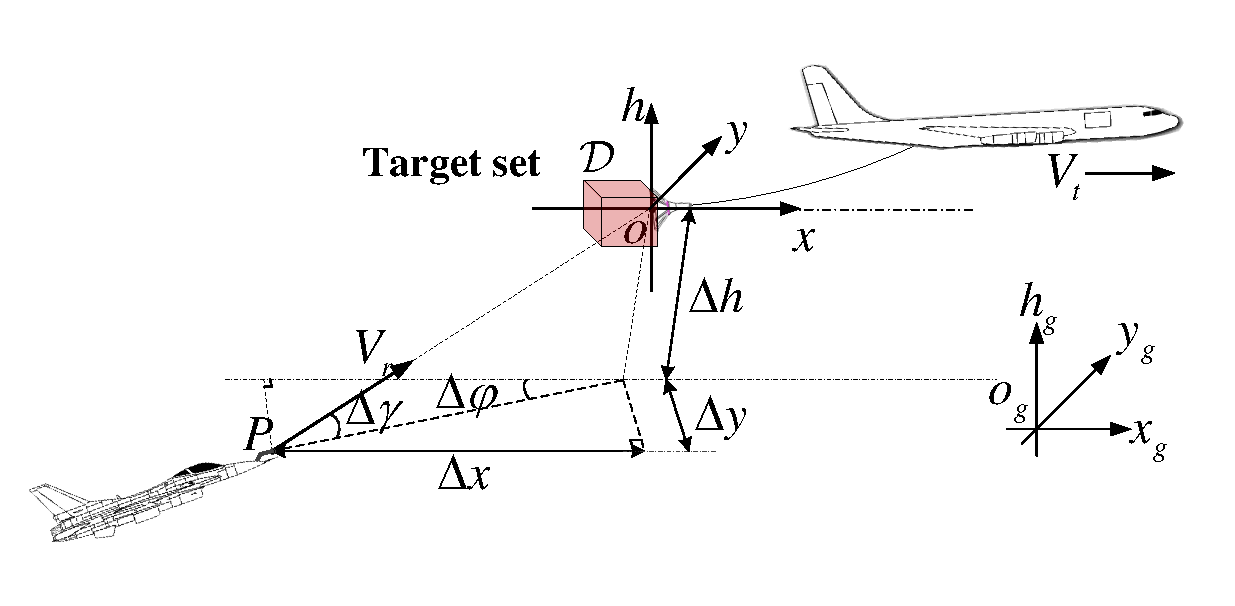
\includegraphics[width=0.5\textwidth]{Figures/Figs_Ch13/Fig1}
		\par\end{centering}
	\caption{The relative position between the receiver and the tanker.}
	\label{Fig1} 
\end{figure}

The relative position between the tip of the probe and the center of the drogue in relative coordinates at the docking phase is considered. At the docking phase, the wind is the main source of the uncertainty on the relative position of the tip of the probe and the center of the drogue. The motions of the tip of the receiver probe and the drogue hauled by the tanker is hauling can be described by the following stochastic differential equations\cite{hu2003aircraft}
\begin{equation}
\label{eq1}
{\rm {d}}{{\mathbf{x}}_\text{r}}\left( t \right) = {\mathbf a}_1\left( t \right){{\rm d} t }  + {\mathbf{f}}\left( {{{\mathbf x}_\text{r}},t} \right){\rm{d}t} + \mathbf \Gamma {\rm d \mathbf B}\left( {{{\mathop{\mathbf x}\nolimits}_\text{r}},t} \right)
\end{equation}
\begin{equation}
\label{eq2}
{\rm {d}}{{\mathbf{x}}_\text{t}}\left( t \right) = {\mathbf a}_2\left( t \right){{\rm d} t }  + {\mathbf{f}}\left( {{{\mathbf x}_\text{t}},t} \right){\rm{d}t} + \mathbf \Gamma {\rm d \mathbf B}\left( {{{\mathop{\mathbf x}\nolimits}_\text{t}},t} \right)
\end{equation}
where the state vector $ {\mathbf x_\text{r}} = {[\begin{array}{*{20}{c}}{{{\mathop{ x}\nolimits} _\text{r}}}&{{y_\text{r}}}&{{h_\text{r}}}\end{array}]^{\text{T}}} $ represents the longitudinal distance, latitudinal distance and altitude of the tip of the probe in the earth-fixed coordinate system, and $ {\mathbf x_\text{t}} = {[\begin{array}{*{20}{c}}
	{{{\mathop{ x}\nolimits} _\text{t}}}&{{y_\text{t}}}&{{h_\text{t}}}
	\end{array}]^{\text{T}}} $   represents the longitudinal distance, latitudinal distance and altitude of the center of the drogue in the earth-fixed coordinate system. Functions $ {{\mathop{\mathbf a}\nolimits}_1}:\left[ {0,\infty } \right) \to {\mathbb{R}^3} $ and $ {{\mathop{\mathbf a}\nolimits}_2}:\left[ {0,\infty } \right) \to {\mathbb{R}^3} $  represent the kinematic states of the tip of the probe and the drogue in the earth-fixed coordinate system. Concretely,  $ {\mathbf a}_1\left( t \right) $ represents the kinematic equation of the probe in the earth-fixed coordinate system, and  $ {\mathbf a}_2\left( t \right) $  represents the kinematic equation of the drogue in the earth-fixed coordinate system. Due to the tanker always in steady flight with a constant speed $ V_\text{t} $ at the docking phase,  $ {\mathbf a}_1\left( t \right) $  and  $ {\mathbf a}_2\left( t \right) $  satisfy
\[{{\mathop{\mathbf a}\nolimits} _1}\left(  t \right) = \left[ {\begin{array}{*{20}{c}}
	{{V_\text{r}}\left( t \right)\cos {\gamma _\text{r}}\left( t \right)\cos {\varphi _\text{r}}\left( t \right)}\\
	{{V_\text{r}}\left( t \right)\cos {\gamma _\text{r}}\left( t \right)\sin {\varphi _\text{r}}\left( t \right)}\\
	{{V_\text{r}}\left( t \right)\sin {\gamma _\text{r}}\left( t \right)}
	\end{array}} \right], \quad {{\mathop{\mathbf a}\nolimits} _2}\left( t \right) \equiv \left[ {\begin{array}{*{20}{c}}
	{{V_\text{t}}}\\
	0\\
	0
	\end{array}} \right].
\]

The function $ {{\mathop{\mathbf f}\nolimits}}:{\mathbb{R}^3} \times  \left[ {0,\infty } \right) \to {\mathbb{R}^3} $ represents the wind field. The function  $ {\mathbf f}\left( \mathbf x,t \right) $ is affine transformation in  $ \mathbf  x $ and can be represented as $ {\mathbf f}\left( \mathbf x,t \right)=\mathbf r\left( t \right)\mathbf{x}+\mathbf l \left( t \right) $, where  $ {{\mathop{\mathbf r}\nolimits}}: \left[ {0,\infty } \right) \to {\mathbb{R}^{3 \times 3}}, {{\mathop{\mathbf l}\nolimits}}: \left[ {0,\infty } \right) \to {\mathbb{R}^{3 }}  $. The matrix $\mathbf \Gamma  $  is used to change the variance of the random perturbation. To simplify the problem,  $ \mathbf \Gamma  $  is assumed to be a constant diagonal matrix given by $ \mathbf \Gamma = {\rm{diag}}\left( {{\sigma _1},{\sigma _2},{\sigma _3}} \right),{\sigma _1},{\sigma _2},{\sigma _3} > 0 $. The function  $ {{\mathop{\mathbf B}\nolimits}}:{\mathbb{R}^3}\times\left[ {0,\infty } \right) \to {\mathbb{R}^3} $  denotes stochastic perturbation, $ {\mathbf B}\left( \mathbf x,t \right) $ is not a standard Brownian motion but a function related to the current state $ \mathbf x $. However,  $ {\mathbf B}\left( \mathbf x_0,t \right) $  is a standard Brownian motion for a specific position ${{\mathop{\mathbf x}\nolimits} _0} \in \mathbb{R}^3 $.  The covariance of $ {\mathop{\mathbf B}\nolimits} \left( \cdot \right) $ can be represented as\cite{hu2005aircraft}
\begin{equation}
\label{eq3}
E\left( {\left( {{\bf{B}}\left( {{{\bf{x}}_1},{t_2}} \right) - {\bf{B}}\left( {{{\bf{x}}_1},{t_1}} \right)} \right){{\left( {{\bf{B}}({{\bf{y}}_1},{t_2}) - {\bf{B}}\left( {{{\bf{y}}_1},{t_1}} \right)} \right)}^{\text{T}}}} \right) = \rho \left( {{{\bf{x}}_1} - {{\bf{y}}_1}} \right)\left( {{t_1} - {t_2}} \right){{\mathop{\mathbf I}\nolimits} _3} \quad {{\bf{x}}_1}, {{\bf{y}}_1} \in \mathbb{R} {^3}\quad{t_1} < {t_2}
\end{equation}
where $ {{\bf{x}}_1} $ and ${{\bf{y}}_1} $  represent the position of the tip of probe and center of the drogue,  $ { \bf I_3} $ represents the 3-by-3 identity matrix and $ \rho : \mathbb{R}^3 \to  \mathbb{R}  $ represents the spatial correlation function. Supposing that the drogue is in the same position as the tip of the probe, namely $ {{{\bf{x}}_1} - {{\bf{y}}_1}=0} $ , then $ \rho \left( {{{\bf{x}}_1} - {{\bf{y}}_1}} \right) = 1 $; if the distance between probe and drogue is infinite, then $ \rho \left( {{{\bf{x}}_1} - {{\bf{y}}_1}} \right) = 0 $. It means that the closer the tip of the probe and the center of the drogue are in the space, the more similar the wind speeds at the two positions are. If the tip of the probe and the center of the drogue move farther away from each other, the wind speeds of the two positions become more independent.

Subtracting Eq. (\ref{eq2}) from Eq. (\ref{eq1}), the relative position of the tip of the probe and the center of the drogue is written as 
\begin{equation}
\label{eq4}
{\rm{d}}{{\bf{\tilde x}}_\text{r/t}}\left( t \right) = {\bf{u}}\left( t \right){\rm{d}}t + {{r}}\left(  t \right){{\bf{\tilde x}}_\text{r/t}}\left( t \right){\rm{d}}t + \mathbf \Gamma {\rm{d}}{\bf{z}}\left( t \right)
\end{equation}
where ${{\bf{\tilde x}}_\text{r/t}}= \bf x_\text{r} - \bf x_\text{t}  $ and $ {{\bf{\tilde x}}_\text{r/t}}={\left[ {\Delta x\Delta y\Delta h} \right]^\text T} $ represents the longitudinal distance, latitudinal distance and altitude of the tip of the probe with respect to the center of the drogue, respectively; $ \mathbf u \left( t \right)=\mathbf{a}_1\left( t \right) - \mathbf{a}_2\left( t \right) $ represents the kinematic states of the tip of the probe with respect to the center of the drogue. Based on Eq. (\ref{eq3}), define $ {\bf{z}}\left( t \right) = {\bf{B}}\left( {{{\bf{x}}_\text{r}},t} \right) - {\bf{B}}\left( {{{\bf{x}}_\text{t}},t} \right) $, where $ {\bf{z}}\left( t \right) $ is a Gaussian process with the covariance 
\begin{equation}
\label{eq5}
E\left({\left( {{\bf{z}}\left( {{t_2}} \right) - {\bf{z}}\left( {{t_1}} \right)} \right){{\left( {{\bf{z}}\left( {{t_2}} \right) - {\bf{z}}\left( {{t_1}} \right)} \right)}^{\text{T}}}} \right) = 2\left( {1 - \rho \left( {{{{\mathbf{\tilde x}}}_\text{r/t}}} \right)} \right)\left( {{t_2} - {t_1}} \right){{\mathbf I}_3}\quad {t_1} < {t_2}
\end{equation}
The concrete proof of Eq. (\ref{eq5}) is presented in Appendix.

According to Eq. (\ref{eq5}), one can get  $ z\left( t \right) = \sqrt {2\left( {1 - \rho \left( {{{{\bf{\tilde x}}}_\text{r/t}}} \right)} \right)} {\bf{W}}\left( t \right) $. Then, Eq. (\ref{eq4}) is rewritten as
\begin{equation}
\begin{aligned}
{\rm{d}}{{{\bf{\tilde x}}}_\text{r/t}}\left( t \right) &= {\bf{u}}\left( t \right){\rm{d}}t + {\bf{r}}\left( t \right){{{\bf{\tilde x}}}_\text{r/t}}\left( t \right){\rm{d}}t + \sqrt {2\left( {1 - \rho \left( {{{{\bf{\tilde x}}}_\text{r/t}}} \right)} \right)} \mathbf \Gamma {\rm{d}}{\bf{W}}\left( t \right)\\
&= \left( {{\bf{u}}\left( t \right) + r\left( t \right){{{\bf{\tilde x}}}_\text{r/t}}\left( t \right)} \right){\rm{d}}t + \sqrt {2\left( {1 - \rho \left( {{{{\bf{\tilde x}}}_\text{r/t}}} \right)} \right)}\mathbf \Gamma {\rm{d}}{\bf{W}}\left( t \right)\\
&= \alpha \left( {{{{\bf{\tilde x}}}_\text{r/t}},t} \right){\rm{d}}t + \beta \left( {{{{\bf{\tilde x}}}_\text{r/t}}} \right)\mathbf\Gamma {\rm{d}}{\bf{W}}\left( t \right)
\label{eq6}
\end{aligned}
\end{equation}  
where $ \mathbf W\left( t \right) $  is a standard 3D Brownian motion, $ \alpha \left( {{{{\bf{\tilde x}}}_\text{r/t}},t} \right)= \mathbf u\left( t \right)+\mathbf r\left( t \right){{\bf{\tilde x}}}_\text{r/t} $  is the drift term and $ \beta \left( {{{{\bf{\tilde x}}}_\text{r/t}}} \right)= \sqrt {2\left( {1 - \rho \left( {{{{\bf{\tilde x}}}_\text{r/t}}}\right)} \right)} $ represents the diffusion term. Eq. (\ref{eq6}) is a standard stochastic differential equation. According to Eq. (6), the relative motion model between the center of the drogue and the tip of the probe is expressed as
\begin{equation}
\label{eq7}
{\rm{d}}\left[ {\begin{array}{*{20}{c}}
	{\Delta x}\\
	{\Delta y}\\
	{\Delta h}
	\end{array}} \right] = \left[ {\begin{array}{*{20}{c}}
	{ - {V_\text{t}} + {V_\text{r}}\left( t \right)\cos {\gamma _\text{r}}\left( t \right)\cos {\varphi _\text{r}}\left( t \right)}\\
	{{V_\text{r}}\left( t \right)\cos {\gamma _\text{r}}\left( t \right)\sin {\varphi _\text{r}}\left( t \right)}\\
	{{V_\text{r}}\left( t \right)\sin {\gamma _\text{r}}\left( t \right)}
	\end{array}} \right]{\rm{d}}r + {\bf{r}}\left( t \right)\left[ {\begin{array}{*{20}{c}}
	{\Delta x}\\
	{\Delta y}\\
	{\Delta h}
	\end{array}} \right]{\rm{d}}t + \sqrt {2\left[ {1 - \rho \left( {{{{\bf{\tilde x}}}_\text{r/t}}} \right)} \right]} \left[ {\begin{array}{*{20}{c}}
	{{\sigma _ h}}&0&0\\
	0&{{\sigma _ h}}&0\\
	0&0&{{\sigma _ v}}
	\end{array}} \right]{\rm{d}}{\bf{W}}\left( t \right)
\end{equation}
Here, $ {{\bf{\tilde x}}}_\text{r/t} $ is restricted by state constraint $ 
\chi  \subset \mathbb{R}^3  $, where $ \chi $ represents the feasible position of the tip of the probe with respect to the center of the drogue at the docking phase. The speed of the tanker is constant and the control variable is the state parameters of the receiver namely $ V_{r} $, $ {\gamma _\text{r}}  $ and $ \varphi _\text{r}  $ at the docking phase. The values $ \sigma _ h $  and  $ \sigma _ v $ are adopted to describe the variation of stochastic perturbation. The larger the values are, the larger the variation in perturbation of the corresponding dimension is.

The spatial correlation function  $ \rho \left( {\mathbf{\tilde x}}_\text{r/t}\right)  $ can be expressed as\cite{liang2013resampling}
\begin{equation}
\begin{aligned}
\rho \left( {{{{\mathbf{\tilde x}}}_\text{r/t}}} \right) = \exp \left( { - {c_h}{{\left\| {{{{\mathbf{\tilde x}}}_\text{r/t}}} \right\|}_ h} - {c_ v}{{\left\| {{{{\mathbf{\tilde x}}}_\text{r/t}}} \right\|}_ v}} \right)
\label{eq8}
\end{aligned}
\end{equation} 
where $ {c_ h>0} $  and  $ {c_ v>0} $  represent the longitudinal correlation coefficient and latitudinal correlation coefficient. If $ {c_ h> c_ v} $, then the correlation of the wind perturbations in the vertical direction is greater than that in the horizontal plane. In Eq. (\ref{eq7}), one has
\begin{equation}
\begin{aligned}
{\left\| {{{{\mathbf{\tilde x}}}_\text{r/t}}} \right\|_ h} = \sqrt {\Delta {x^2} + \Delta {y^2}} ,{\left\| {{{{\mathbf{\tilde x}}}_\text{r/t}}} \right\|_ v} = \left| {\Delta h} \right|
\label{eq9}
\end{aligned}
\end{equation} 

A neighborhood around the desired final states at the docking phase is defined as the target set $ {\cal D} $. For the relative motion model Eq. (\ref{eq7}), the target set $ {\cal D} $ is a cube.

\textbf{Definition 1:}  Given a target set $ {\cal D} $, the probability of docking success for the initial state $ {{{{\mathbf{\tilde x}}}_\text{r/t}}} $  at the docking phase over the time horizon $ t \in \left[ {0,t_f } \right] $  is
\begin{equation}
\begin{aligned}
P \buildrel \Delta \over = P\left\{ {{\mathbf {\tilde x}_\text{r/t}}\left( {{t_f}} \right) \in {\cal D}|{\mathbf {\tilde x}_\text{r/t}}\left( 0 \right) \in {\cal X},t \in \left[ {0,{t_f}} \right]} \right\}
\label{eq10}
\end{aligned}
\end{equation} 
which satisfies the state constraint Eq. (\ref{eq7}), where $ t_f>0 $ represents the end time of the docking phase.

\section{Docking Success Probability Evaluation}\label{section3}
To make this paper self-contained, some preliminary results on the stochastic approximation method is recalled firstly. Then the computing procedure of the probability of docking success is provided.

\subsection{General ideas}
The objective is to determine the probability of docking success of the states at the docking phase, as shown in Eq. (\ref{eq10}). The stochastic approximation method is adopted to evaluate the probability of docking success based on the Markov chain approximation scheme, where the Cartesian grid is used to approximate the state space in the Markov chain. It is necessary to consider the uncertainty of state transition due to the stochastic perturbations.

The general ideas of determining the probability of docking success of the states using the stochastic approximation method are described in the following. 

$ \bullet $ First, determine the state space during the docking phase. The state space set is divided into three sets, which are the target set $ {\cal D} $, the state constraint set $ \chi $, and the state space which is outside the target set but inside $ \chi $ can be denoted by $ {\cal L} = {{\cal X} \mathord{\left/
		{\vphantom {{\cal X} {\cal D}}} \right.
		\kern-\nulldelimiterspace} {\cal D}} $.

$ \bullet $ Second, discretize the state space. Divide the state space $ {\cal L} $ into grids, with the grid size being $\delta  > 0 $. The set of grids $ Q $ in the state space $ {\cal L} $ is further divided into boundary grids $ \partial {Q_{\cal L}} = \partial {Q_{\cal X}} \cup \partial {Q_{\cal D}} $  and interior grids ${Q_0} = {Q \mathord{\left/
		{\vphantom {Q {\partial {Q_{\cal L}}}}} \right.
		\kern-\nulldelimiterspace} {\partial {Q_{\cal L}}}} $. The state space and its partition are shown in Fig. \ref{Fig2}.

$ \bullet $ Third, define the Markov chain ${Q_k} $. Based on the discretization of the state space, the probability of the current grid point $ q $ transferring to the adjacent grid point set $ {{\cal N}_q} $ and to the grid point itself is described by using the transition probability of Markov chain. For interior grid points $ q \in {Q_0} $, its adjacent grid point set is $ {{\cal N}_q} $. For the three-dimensional state equation shown in equation (\ref{eq7}), the state transition from the current grid point $ q $ to the adjacent grid point set $ {{\cal N}_q}  $ and to the grid point itself can be described by Fig. \ref{Fig3}. As shown in \ref{Fig3}, the adjacent grid point set of q includes $ {q_{1 + }} $, $ {q_{1 - }} $, $ {q_{2 + }} $, $ {q_{2 - }} $ , $ {q_{3 + }} $  and $ {q_{3 - }} $, which are specifically expressed as $ {q_{i + }} = {q_{i + }} + {\eta _i}\delta  $  and $ {q_{i - }} = {q_{i - }} + {\eta _i}\delta $  ($i = 1,2,3 $ ). Here, $ {\eta _i} $  ($i = 1,2,3 $ ) are related to the parameters in the constant diagonal matrix $ {\bf{\Gamma }} $ and specifically expressed as ${\eta _i} = {{{\sigma _i}} \mathord{\left/
		{\vphantom {{{\sigma _i}} {\bar \sigma }}} \right.
		\kern-\nulldelimiterspace} {\bar \sigma }} $ ($i = 1,2,3 $ ), where ${\sigma _1} = {\sigma _2} = {\sigma _h} $ , $ {\sigma _3} = {\sigma _v} $ and $ \bar \sigma  = \max {\sigma _i} $.

$ \bullet $ Fourth, the probability of docking success of the corresponding grid points in the state space $ {\cal L} $ are finally obtained by appropriately propagating the transition probabilities of the Markov chain backward starting from the target set.


\begin{figure}[H]
	\begin{minipage}[t]{0.5\textwidth}
		\centering
		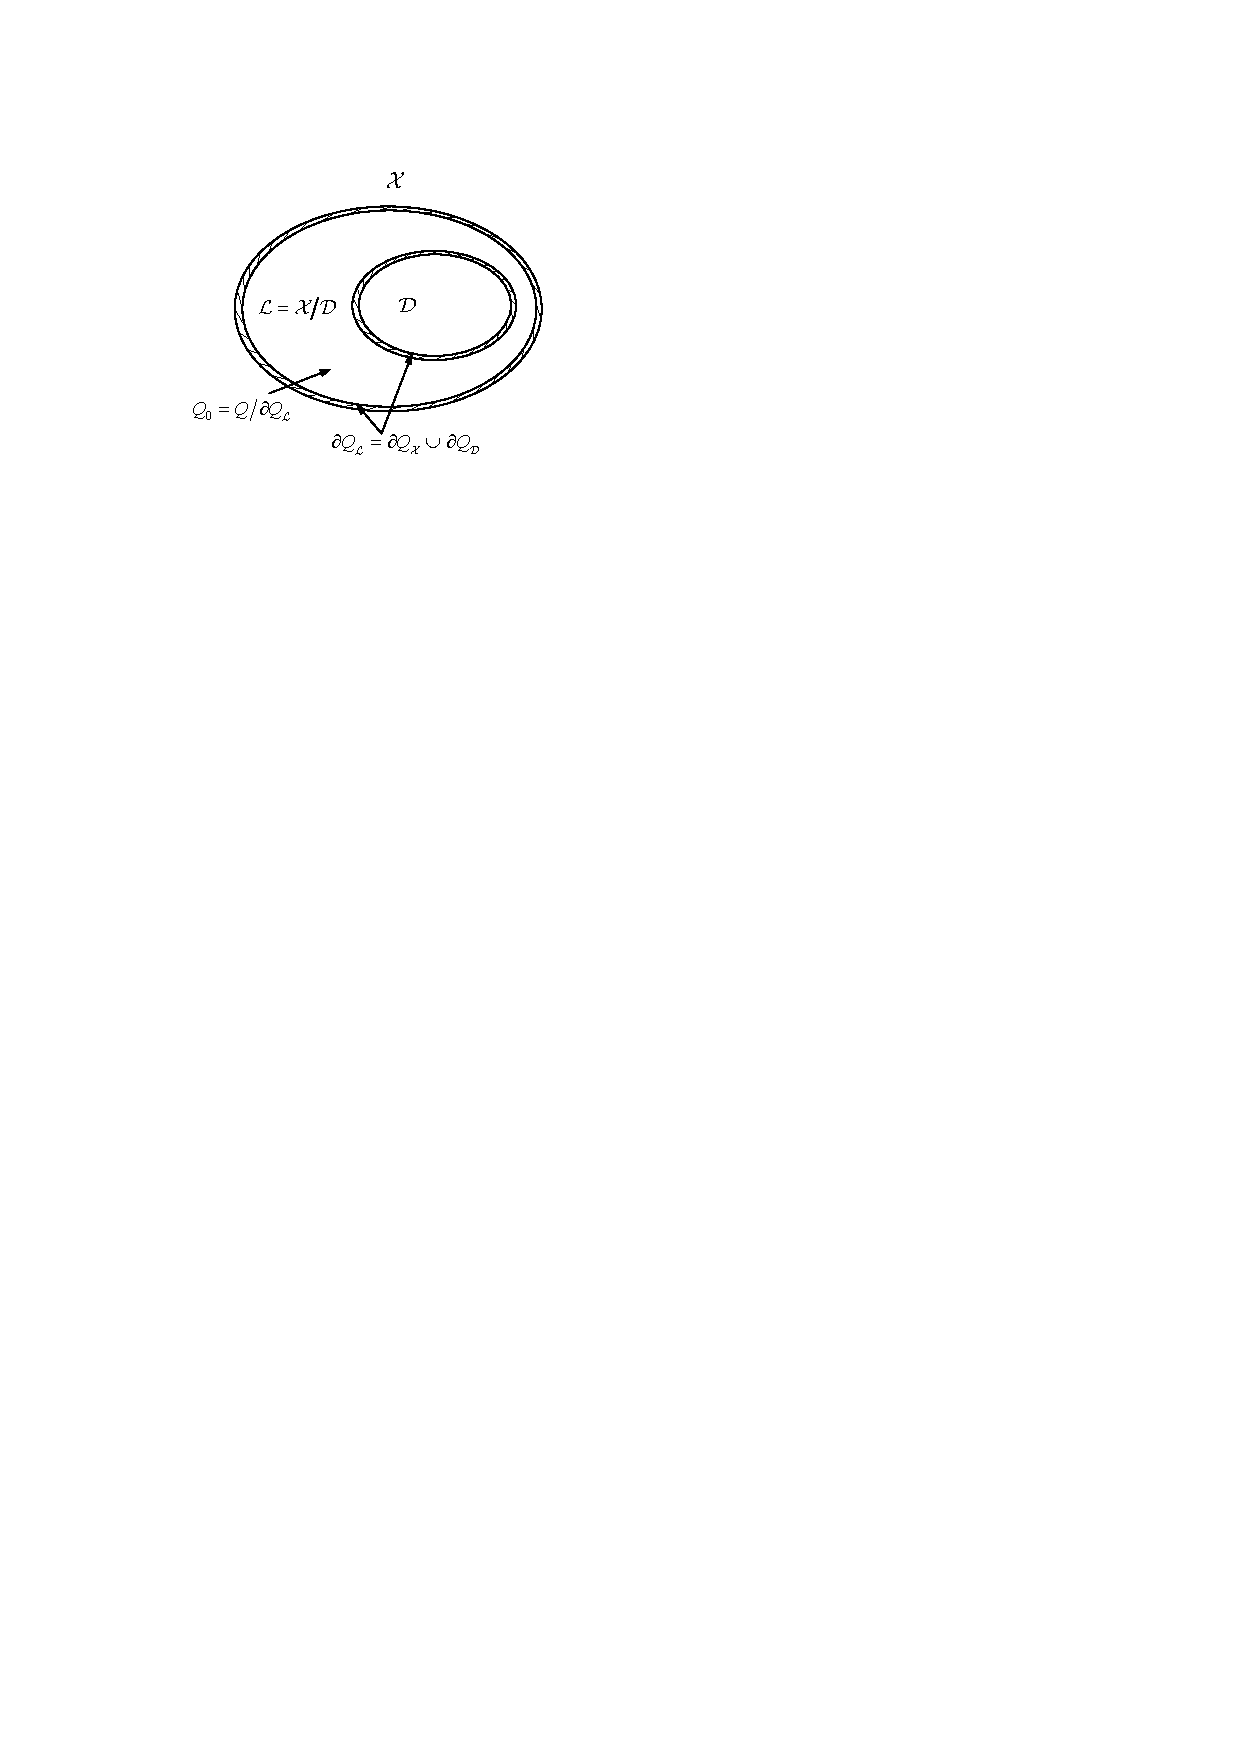
\includegraphics[scale=0.8]{Figures/Figs_Ch13/Fig2}
		\caption{State space and its partition.\label{Fig2}}
	\end{minipage}
	\qquad
	\begin{minipage}[t]{0.4\textwidth}
		\centering
		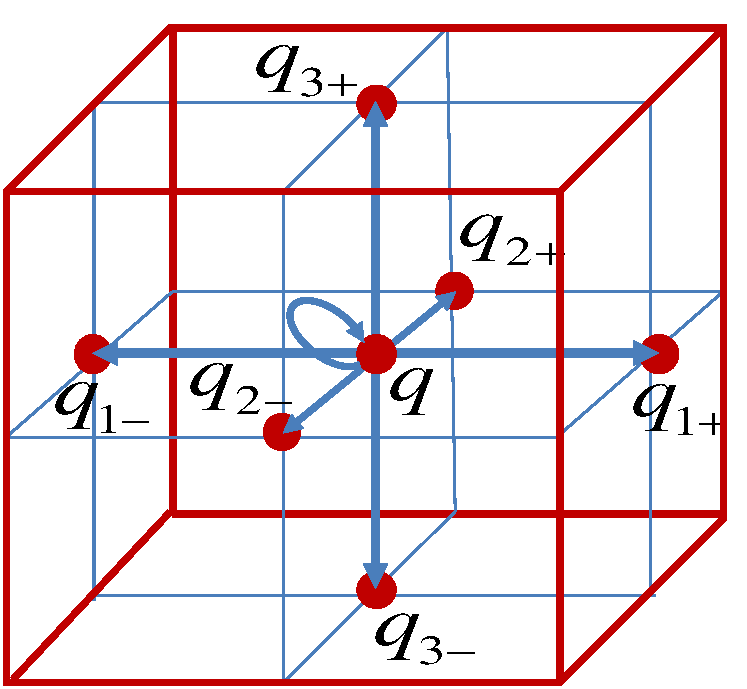
\includegraphics[scale=0.3]{Figures/Figs_Ch13/Fig3}
		\caption{Graph description of state transition.\label{Fig3}}
	\end{minipage}
\end{figure}

\subsection{The transition probability of Markov chain}
The transition probability of Markov chain is used in stochastic approximation method to describe the change of the states. It is provided as follows\cite{sinha1971stochastic}:\\
(1) If  $ q \in \partial {Q_{\cal L}} $, the transition probability is expressed as
\begin{equation}
\begin{aligned}
P\left\{ {{Q_{k + 1}} = q'|{Q_k} = q} \right\} = \left\{ \begin{array}{l}
1{\kern 1pt} {\kern 1pt} {\kern 1pt} {\kern 1pt} {\kern 1pt} {\kern 1pt} {\kern 1pt} {\kern 1pt} {\kern 1pt} {\kern 1pt} {\kern 1pt} {\kern 1pt} {\kern 1pt} {\kern 1pt} {\kern 1pt} {\kern 1pt} {\kern 1pt} {\kern 1pt} {\kern 1pt} q' = q{\kern 1pt} {\kern 1pt} {\kern 1pt} {\kern 1pt} {\kern 1pt} {\kern 1pt} {\kern 1pt} {\kern 1pt} {\kern 1pt} {\kern 1pt} {\kern 1pt} {\kern 1pt} {\kern 1pt} {\kern 1pt} {\kern 1pt} \\
0{\kern 1pt} {\kern 1pt} {\kern 1pt} {\kern 1pt} {\kern 1pt} {\kern 1pt} {\kern 1pt} {\kern 1pt} {\kern 1pt} {\kern 1pt} {\kern 1pt} {\kern 1pt} {\kern 1pt} {\kern 1pt} {\kern 1pt} {\kern 1pt} {\kern 1pt} {\kern 1pt} otherwise{\kern 1pt} {\kern 1pt} {\kern 1pt} 
\end{array} \right.
\label{eq11}
\end{aligned}
\end{equation}
The grid point q will not transfer to another grid point, as the set $  \partial {Q_{\cal L}} $ is an absorbing region.

(2)	If  $ q \in {Q_0} $, the transition probability from the grid point $ q $ to the adjacent grid $ q' \in {{\cal N}_q} $ is expressed by
\begin{equation}
\begin{aligned}
P\left\{ {{Q_{k + 1}} = q'|{Q_k} = q} \right\} = \left\{ \begin{array}{l}
p_{q'}^k\left( q \right){\kern 1pt} {\kern 1pt} {\kern 1pt} {\kern 1pt} {\kern 1pt} {\kern 1pt} {\kern 1pt} {\kern 1pt} {\kern 1pt} {\kern 1pt} q' \in {{\cal N}_q} \cup \left\{ q \right\}{\kern 1pt} \\
0{\kern 1pt} {\kern 1pt} {\kern 1pt} {\kern 1pt} {\kern 1pt} {\kern 1pt} {\kern 1pt} {\kern 1pt} {\kern 1pt} {\kern 1pt} {\kern 1pt} {\kern 1pt} {\kern 1pt} {\kern 1pt} {\kern 1pt} {\kern 1pt} {\kern 1pt} {\kern 1pt} {\kern 1pt} {\kern 1pt} {\kern 1pt} {\kern 1pt} {\kern 1pt} {\kern 1pt} {\kern 1pt} {\kern 1pt} {\kern 1pt} {\kern 1pt} {\kern 1pt} {\kern 1pt} {\kern 1pt} {\kern 1pt} {\kern 1pt} {\kern 1pt} otherwise{\kern 1pt} {\kern 1pt} {\kern 1pt} {\kern 1pt} {\kern 1pt} {\kern 1pt} {\kern 1pt} {\kern 1pt} {\kern 1pt} {\kern 1pt} {\kern 1pt} {\kern 1pt} {\kern 1pt} {\kern 1pt} 
\end{array} \right.
\label{eq12}
\end{aligned}
\end{equation}
where $p_{q'}^k\left( q \right) $ represents the probability of transition from the grid point $ q $ to the grid point $ q' $ in the $ k $-th step. For the discrete state space, the drift term and diffusion term can be denoted by $ \alpha \left( {q,k\Delta t} \right) $ and $ \beta \left( q \right) $ respectively, where $ \Delta t $ represents the time step. Thus, $ p_{q'}^k\left( q \right) $ can be expressed by
\begin{equation}\label{eq13}
p_{q'}^k\left( q \right) = \left\{ \begin{array}{l}
p_q^k\left( q \right) = \frac{{\xi _0^k\left( q \right)}}{{C_q^k}},{\kern 1pt} {\kern 1pt} {\kern 1pt} q' = q\\
p_{{q_{i + }}}^k\left( q \right) = \frac{{\exp \left( {\delta \xi _i^k\left( q \right)} \right)}}{{C_q^k}},{\kern 1pt} {\kern 1pt} {\kern 1pt} q' = {q_{i + }},i = 1,2,3\\
p_{{q_{i - }}}^k\left( q \right) = \frac{{\exp \left( { - \delta \xi _i^k\left( q \right)} \right)}}{{C_q^k}},{\kern 1pt} {\kern 1pt} {\kern 1pt} q' = {q_{i - }},i = 1,2,3
\end{array} \right.
\end{equation}
where
\[\xi _0^k\left( q \right) = \frac{2}{{\lambda {{\bar \sigma }^2}\beta {{\left( q \right)}^2}}} - 2n{\kern 1pt} ,{\rm{ }}\xi _i^k\left( q \right) = \frac{{{{\left( {\alpha \left( {q,k\Delta t} \right)} \right)}_i}}}{{{\eta _i}{{\bar \sigma }^2}\beta {{\left( q \right)}^2}}}{\kern 1pt} ,{\kern 1pt} {\rm{ }}C_q^k = \sum\limits_{i = 1}^3 {\left( {\exp \left( {\delta \xi _i^k\left( q \right)} \right) + \exp \left( { - \delta \xi _i^k\left( q \right)} \right)} \right)}  + \xi _0^k\left( q \right)\]
and $ \lambda  $ is a positive constant. Here, according to Eq. (\ref{eq7}), the definitions of $\alpha \left( {q,k\Delta t} \right),\beta \left( q \right) $ are
\[\alpha \left( {q,k\Delta t} \right) = \left[ \begin{array}{l}
- {V_\text{t}} + {V_\text{r}}\left( {k\Delta t} \right)\cos {\gamma _\text{r}}\left( {k\Delta t} \right)\cos {\varphi _\text{r}}\left( {k\Delta t} \right)\\
{\kern 1pt} {\kern 1pt} {\kern 1pt} {\kern 1pt} {\kern 1pt} {\kern 1pt} {\kern 1pt} {\kern 1pt} {\kern 1pt} {\kern 1pt} {\kern 1pt} {\kern 1pt} {\kern 1pt} {V_\text{r}}\left( {k\Delta t} \right)\cos {\gamma _\text{r}}\left( {k\Delta t} \right)\sin {\varphi _\text{r}}\left( {k\Delta t} \right){\kern 1pt} {\kern 1pt} {\kern 1pt} {\kern 1pt} {\kern 1pt} {\kern 1pt} {\kern 1pt} {\kern 1pt} {\kern 1pt} \\
{\kern 1pt} {\kern 1pt} {\kern 1pt} {\kern 1pt} {\kern 1pt} {\kern 1pt} {\kern 1pt} {\kern 1pt} {\kern 1pt} {\kern 1pt} {\kern 1pt} {\kern 1pt} {\kern 1pt} {\kern 1pt} {\kern 1pt} {\kern 1pt} {\kern 1pt} {\kern 1pt} {\kern 1pt} {\kern 1pt} {\kern 1pt} {\kern 1pt} {\kern 1pt} {\kern 1pt} {\kern 1pt} {V_\text{r}}\left( {k\Delta t} \right)\sin {\gamma _\text{r}}\left( {k\Delta t} \right)
\end{array} \right] + {\bf{r}}\left( {k\Delta t} \right)\left[ \begin{array}{l}
\Delta x\left( {k\Delta t} \right)\\
\Delta y\left( {k\Delta t} \right)\\
\Delta h\left( {k\Delta t} \right)
\end{array} \right]{\kern 1pt} {\kern 1pt} {\kern 1pt}\]
and $ \beta \left( q \right) = \sqrt {2\left( {1 - \rho \left( {{{\tilde x}_\text{r/t}}\left( {k\Delta t} \right)} \right)} \right)}  $.

To ensure the accuracy of the calculation, the time step $\Delta t $ is determined by the constant  $ \lambda  $  and the grid size $ \delta  $, namely $ \Delta t = \lambda {\delta ^2} $.The reference\cite{kurzhanskiy2007ellipsoidal} has proved that the Markov chain mentioned converges weakly to the solution of the stochastic differential equation when the grid size $ \delta  \to 0 $. Therefore, Markov chain can be used to approximate the state equation of the system, and the solution of the stochastic differential equation can be approximated by the probability distribution of the state at a certain moment.

\subsection{Computing procedure of the probability of docking success}

In this section, the computing procedure of the backward probability of docking success is provided. At the docking phase, the target set  $ {\cal D} $ is a cube representing the state set of successful docking. The probability of entering the target set $ {\cal D} $ for each grid point is computed by appropriately propagating the transition probabilities of the Markov chain backward starting from the target set during the specified time horizon $ t $. The probability of docking success $ {P^{\left( k \right)}}\left( q \right) $ satisfies the following recursive equation
\begin{equation}\label{eq14}
{P^{\left( k \right)}}\left( q \right) = \left\{ \begin{array}{l}
p_q^k\left( q \right){P^{\left( {k + 1} \right)}}\left( q \right) + \sum\limits_{q' \in {N_q}} {p_{q'}^k\left( q \right)} {P^{\left( {k + 1} \right)}}\left( {q'} \right),{\kern 1pt} {\kern 1pt} {\kern 1pt} q \in {Q_0}\\
1{\kern 1pt} {\kern 1pt} {\kern 1pt} {\kern 1pt} {\kern 1pt} {\kern 1pt} {\kern 1pt} {\kern 1pt} {\kern 1pt} {\kern 1pt} {\kern 1pt} {\kern 1pt} {\kern 1pt} {\kern 1pt} q \in \partial {Q_{\cal D}}{\kern 1pt} {\kern 1pt} {\kern 1pt} {\kern 1pt} {\kern 1pt} \\
{\kern 1pt} {\kern 1pt} {\kern 1pt} {\kern 1pt} {\kern 1pt} {\kern 1pt} {\kern 1pt} {\kern 1pt} {\kern 1pt} {\kern 1pt} {\kern 1pt} {\kern 1pt} {\kern 1pt} {\kern 1pt} {\kern 1pt} {\kern 1pt} {\kern 1pt} \\
0{\kern 1pt} {\kern 1pt} {\kern 1pt} {\kern 1pt} {\kern 1pt} {\kern 1pt} {\kern 1pt} {\kern 1pt} {\kern 1pt} {\kern 1pt} {\kern 1pt} {\kern 1pt} q \in \partial {Q_{\cal X}}
\end{array} \right.
\end{equation}
where recursive step  $ k \in \left[ {0,{k_f}} \right] \in Z $, time horizon  $ t \in \left[ {0,{t_f}} \right] $, thus  $ {k_f} = \left\lfloor {{{{t_f}} \mathord{\left/{\vphantom {{{t_f}} {\Delta t}}} \right.
			\kern-\nulldelimiterspace} {\Delta t}}} \right\rfloor  $; $ p_q^k\left( q \right) $  and $ p_{q'}^k\left( q \right) $ represent the transition probability from the grid point $ q $ to itself and to the adjacent grid point $ q' \in {N_q} $ in the $ k $-th step, respectively. ${P^{\left( {k + 1} \right)}}\left( q \right) $ and $ {P^{\left( {k + 1} \right)}}\left( {q'} \right) $ represent the probability transited to the grid point $ q $ and probability transited to the adjacent grid point $ q' \in {N_q} $ in the $ (k+1) $-th step. As $ q \in \partial Q_{\cal D} $  represents the state has reached the boundary of the target set and $\partial Q_{\cal D}  $ is an absorbing region, the probability of docking success is 1 when $ q \in \partial Q_{\cal D} $. As $ q \in \partial {Q_{\cal X}}{\kern 1pt}  $ represents the state has reached the boundary of the state space $ {\cal X} $ and $ \partial {Q_{\cal X}} $ also is an absorbing region, the probability of docking success is 0 when $ q \in \partial {Q_{\cal X}} $. 

The initial condition of Eq. (\ref{eq14}) is
\begin{equation}\label{eq15}
{P^{\left( k \right)}}\left( q \right) = \left\{ \begin{array}{l}
1,{\kern 1pt} {\kern 1pt} {\kern 1pt} {\kern 1pt} {\kern 1pt} {\kern 1pt} {\kern 1pt} {\kern 1pt} {\kern 1pt} {\kern 1pt} {\kern 1pt} if{\kern 1pt} {\kern 1pt} {\kern 1pt} q \in \partial {Q_{\cal D}}\\
0,{\kern 1pt} {\kern 1pt} {\kern 1pt} {\kern 1pt} {\kern 1pt} {\kern 1pt} {\kern 1pt} {\kern 1pt} {\kern 1pt} otherwise
\end{array} \right.
\end{equation}
According to Eq. (\ref{eq14}) (\ref{eq15}), the probability that the state corresponding to any grid points in the state space $ {\cal L} $ enters the target set  $ {\cal D}  $ can be obtained. 

Therefore, the computing procedure of the probability of docking success is as follows.\\
Step 1: Initialize the state space $ {\cal X} $, the target set $ {\cal D}  $ and the state space $ {\cal L} = {{\cal X} \mathord{\left/
		{\vphantom {{\cal X} {\cal D}}} \right.
		\kern-\nulldelimiterspace} {\cal D}} $, determine the grid size $ \delta  $ and discretize the state space.\\
Step 2: Define the initial conditions according to Eq. (\ref{eq15}). \\
Step 3: Obtain ${P^{\left( k \right)}}\left( q \right) $ by backward propagating from initial condition according to Eq. (\ref{eq14}).\\ 
Step 4: Print the probability level curves and the probability isosurface according to $ {P^{{k_f}}}(q) $. 

The flow chart of the computation of the docking success probability based on stochastic approximation method is shown in Fig. \ref{Fig4}.
\begin{figure}[h]
	\begin{centering}
		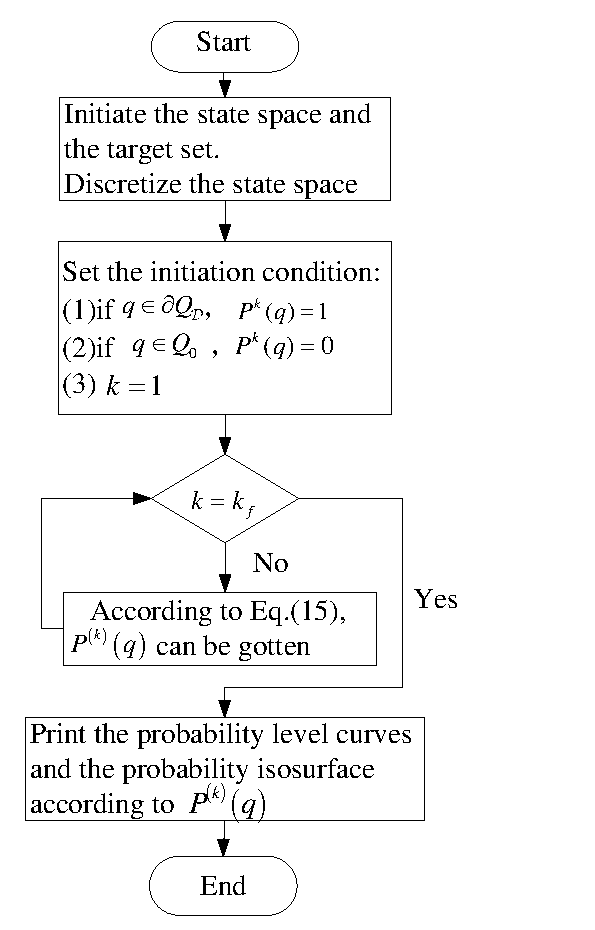
\includegraphics[width=0.3\textwidth]{Figures/Figs_Ch13/Fig4} 
		\par\end{centering}
	\caption{The flow chart of the computation of the docking success probability.}
	\label{Fig4} 
\end{figure}
\section{Simulation analysis on  probability of docking success}\label{section4}
\subsection{Description of the simulation parameters}\label{4.1}
Based on the computing procedure proposed in Section \ref{section3}, the state parameters of Eq. (\ref{eq7}), the state constraint set and the target set at the docking phase are provided.

\textbf{(i)	State parameters}. At the docking phase, the speed of the tanker aircraft is set to be $ {V_\text{t}} = 120  \rm{m/s}  $. The related parameters used in Eq. (\ref{eq13}) is given in Table \ref{table1}. The docking phase is divided into two stages and the time horizon of each stage is 1$ s $. The parameters of each stage are provided in Table \ref{table2}.

\textbf{(ii) State constraint set}. The Cartesian grid is used to approximate the state space $ {\cal X} $. The ranges of the states of the system and the grid division are shown in Table \ref{table3}. If the states are out of the ranges, then the docking is considered to fail. According to the constant $ \lambda $ and the grid size $ \delta  $, the time step is $ \Delta t = \lambda {\delta ^2} = 0.006\rm{s}$. 

\textbf{(iii) Target set}. A neighborhood around the desired final states at the docking phase is chosen as the target set. For the considered system, the target set with respect to $ {\mathbf {\tilde  x}_\text{r/t}} $ is
\begin{equation}\label{eq16}
{\cal D} = \left\{ {{{\mathbf{\tilde x}}_\text{r/t}} \in \mathbb{R}{^3}| - 0.3\rm{m} \le \Delta x \le 0\rm{m}, - 0.5\rm{m} \le \Delta y \le 0.5\rm{m}, - 0.5\rm{m} \le \Delta h \le 0.5\rm{m}} \right\}
\end{equation}

\begin{minipage}{\textwidth}
	
	\begin{minipage}[t]{0.48\textwidth}
		\makeatletter\def\@captype{table}\centering
		\caption{Related parameters of the state equations.}
		\begin{tabular}{c|c}
			\hline
			Paramete     & Value    \\ \hline
			$ t $       & 2$ \rm{s} $        \\ \hline
			$ \lambda $  & 0.15     \\ \hline
			$ c_v $      & 0.2      \\ \hline
			$ c_h $      & 0.05     \\ \hline
			$ \sigma_h $ & 1        \\ \hline
			$ \sigma_v $ & 1        \\
			\hline
		\end{tabular}
		\label{table1}
	\end{minipage}
	\begin{minipage}[t]{0.48\textwidth}
		\makeatletter\def\@captype{table}\centering
		\caption{Parameter values of the two stages.}
		\begin{tabular}{c|cc}
			\hline
			Time interval     & Parameter     & Value  \\
			\hline
			\multirow{3}{*}{	$t \in \left[ {0\rm{s},1\rm{s}} \right]$} & $ V_\text{r} $  & $ 122\rm{m/s} $ \\
			&$ {\gamma _\text{r}}$  & 1     \\
			&  ${\varphi _\text{r}}$      & 1 \\\hline
			\multirow{3}{*}{	$t \in \left[ {1\rm{s},2\rm{s}} \right]$} & $ V_\text{r} $  & $ 125\rm{m / s} $ \\
			&$ {\gamma _\text{r}}$  & 2   \\
			&  ${\varphi _\text{r}}$      & 2 \\                  
			\hline
		\end{tabular}
		\label{table2}
	\end{minipage}
\end{minipage}


\begin{table}[H]
	\centering
	\caption{Grid division of the state space.}
	\begin{tabular}{c|ccc}
		\hline
		Parameter & $\Delta x\left( \rm{m} \right)$ & $\Delta y\left( \rm{m} \right)$ & $\Delta h\left( \rm{m} \right)$ \\
		\hline
		Range & $ \left[ { - 20,1} \right] $ & $ \left[ { - 10,10} \right] $ & $ \left[ { - 10,10} \right] $ \\
		\hline
		Grid numbers & 95 & 100 & 100 \\
		\hline
		Grid size & 0.2 & 0.2 & 0.2 \\
		\hline
	\end{tabular}
	\label{table3}
\end{table} 
\subsection{The probability of docking success\label{4.2}}
The simulation results of the probability of docking success are provided in this section. Specifically, two situa-tions are considered, namely considering the lateral deviation and without considering the lateral deviation.
\subsubsection{Without considering the lateral deviation}

Without considering the lateral deviation, the receiver only needs to adjust the longitudinal distance and altitude deviation between the drogue of the tanker and the probe of the receiver to complete the docking during the dock-ing phase. Thus, Eq. (\ref{eq9}) is rewritten as
\begin{equation}
\begin{aligned}
{\left\| {{{{\bf{\tilde x}}}_\text{r/t}}} \right\|_h} = \left| {\Delta x} \right|,\quad{\left\| {{{{\bf{\tilde x}}}_\text{r/t}}} \right\|_v} = \left| {\Delta h} \right|
\label{eq17}
\end{aligned}
\end{equation}
The wind field is set to be
\begin{equation}
\begin{aligned}
{\bf{r}}\left( {k\Delta t} \right){{\bf{\tilde x}}_\text{r/t}} = \left[ {\begin{array}{*{20}{c}}
	{\frac{1}{5}k\Delta t}&0\\
	0&{ - \frac{1}{5}k\Delta t}
	\end{array}} \right]\left[ {\begin{array}{*{20}{c}}
	{\Delta x}\\
	{\Delta h}
	\end{array}} \right]
\label{eq18}
\end{aligned}
\end{equation}

The probability of docking success is depicted in Fig. \ref{Fig5} when the wind field is not considered, where the numbers on the contour represent the probability of successful docking and the rectangular area with a probability of 1 is the target set. While, the probability of docking success is shown in Fig.6 when the wind field is considered. Comparing Fig. \ref{Fig5} and Fig. \ref{Fig6}, for a given wind field in Eq. (\ref{eq18}), the wind field makes the curves of probability be bent counterclockwise.
\begin{figure}[H]
	\begin{minipage}[t]{0.45\textwidth}
		\centering
		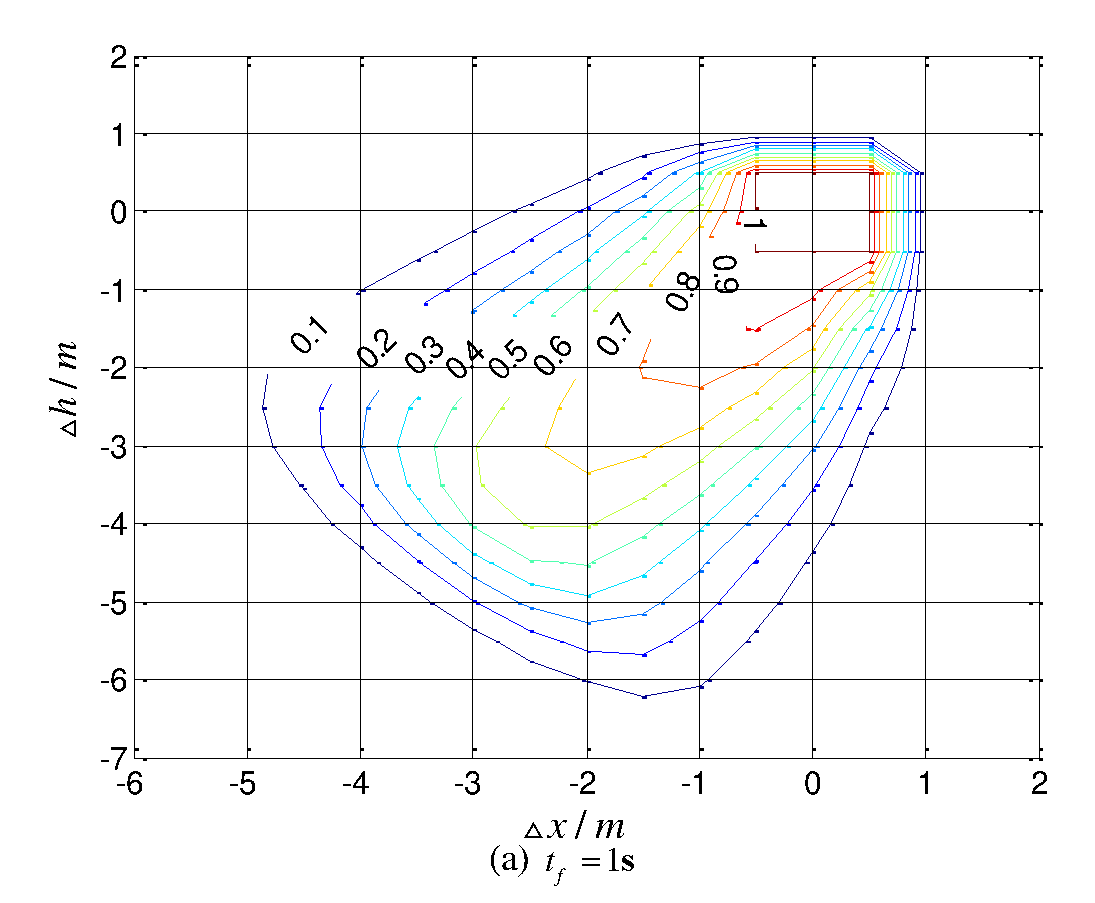
\includegraphics[scale=0.45]{Figures/Figs_Ch13/Fig5_1}		
	\end{minipage}
	\qquad
	\begin{minipage}[t]{0.45\textwidth}
		\centering
		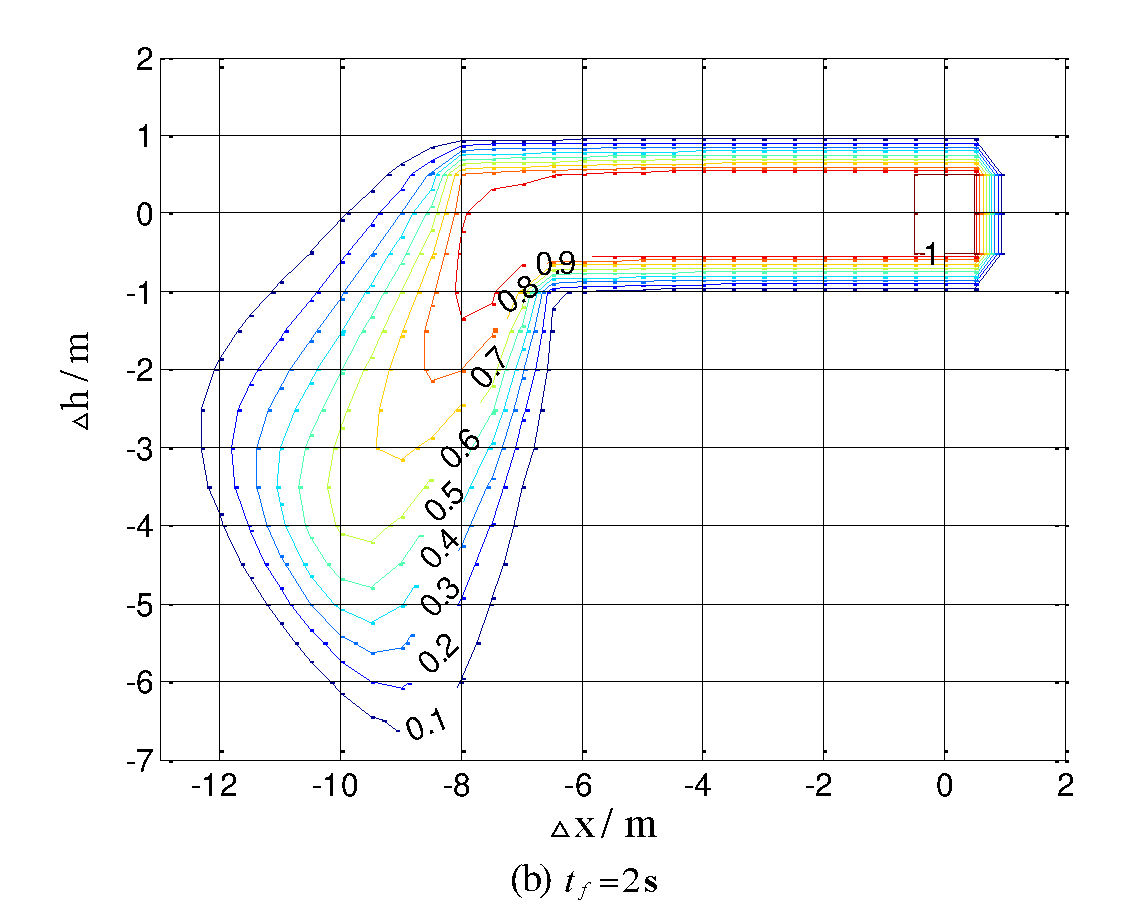
\includegraphics[scale=0.45]{Figures/Figs_Ch13/Fig5_2}
	\end{minipage}
	\caption{Level curves of the probability of docking success without considering wind field.\label{Fig5}}
\end{figure}
\begin{figure}[H]
	\begin{minipage}[t]{0.45\textwidth}
		\centering
		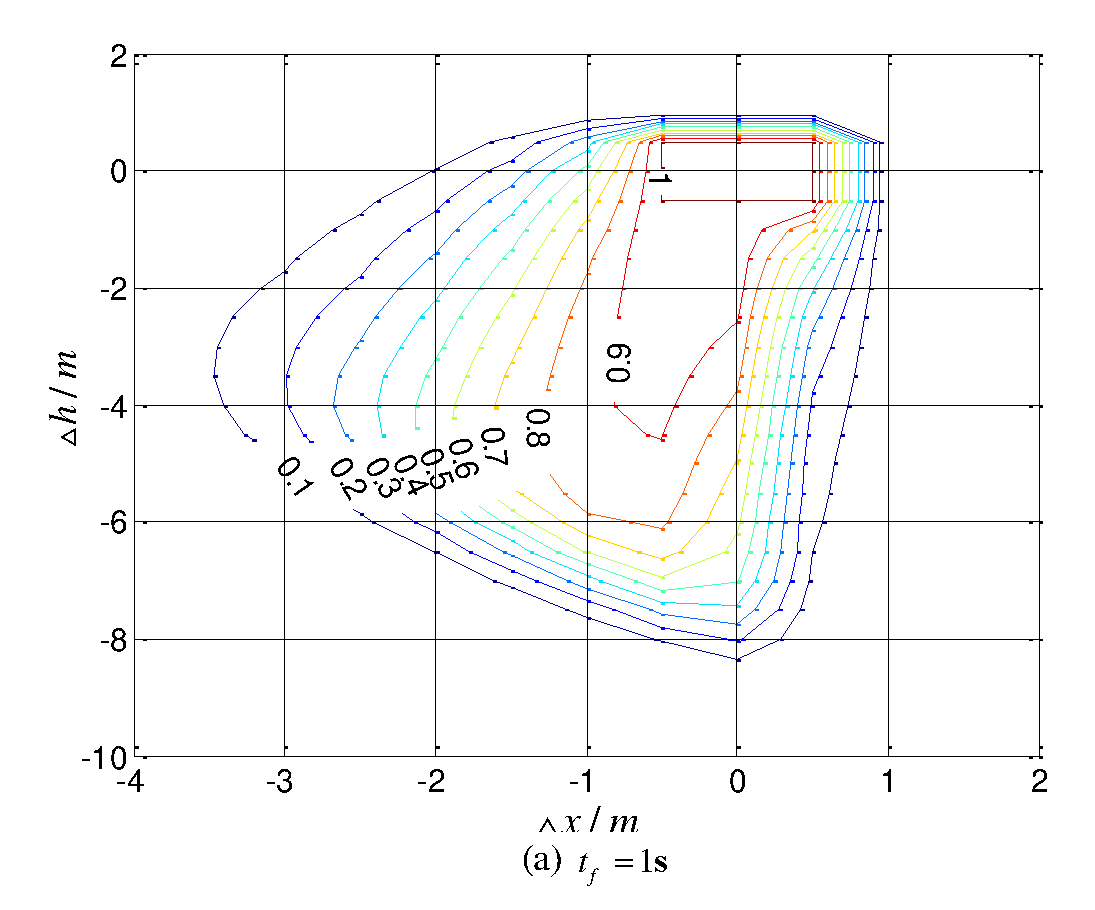
\includegraphics[scale=0.45]{Figures/Figs_Ch13/Fig6_1}		
	\end{minipage}
	\qquad
	\begin{minipage}[t]{0.45\textwidth}
		\centering
		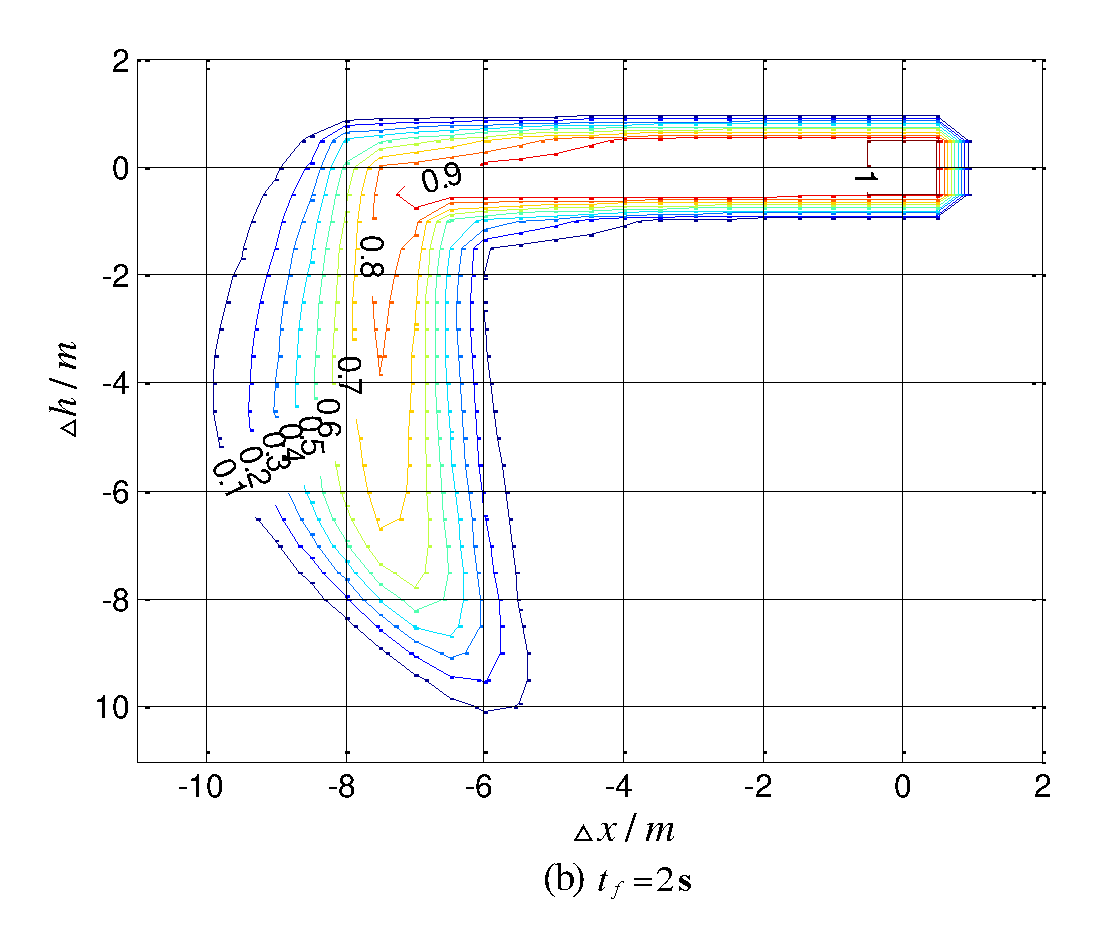
\includegraphics[scale=0.45]{Figures/Figs_Ch13/Fig6_2}
	\end{minipage}
	\caption{Level curves of the probability of docking success without considering wind field.\label{Fig6}}
\end{figure}
\subsubsection{Considering the lateral deviation}

Considering the lateral deviation implies the receiver needs to adjust the longitudinal distance, altitude deviation and lateral deviation between the drogue of the tanker and the probe of the receiver to complete the docking during the docking phase. The wind field is set to be
\begin{equation}
\begin{aligned}
{\bf{r}}(k\Delta t){\mathbf {\tilde x}_\text{r/t}} = \left[ {\begin{array}{*{20}{c}}
	{\frac{1}{5}k\Delta t}&0&0\\
	0&{ - \frac{1}{5}k\Delta t}&0\\
	0&0&{\frac{1}{5}k\Delta t}
	\end{array}} \right]\left[ {\begin{array}{*{20}{c}}
	{\Delta x}\\
	{\Delta y}\\
	{\Delta h}
	\end{array}} \right]
\label{eq19}
\end{aligned}
\end{equation}

The probability of docking success is depicted in Fig. \ref{Fig7} when the wind field is not considered, where the green cube is the target set and the values of the isosurfaces of different colors from inside to outside are 0.2, 0.4, 0.6 and 0.8, respectively. The probability of docking success is depicted in Fig. \ref{Fig8} when the wind field is considered. Comparing Fig. \ref{Fig7} and Fig. \ref{Fig8}, the 3D wind field has the effect on the isosurface of the probability. The range of the probability of docking success with the isosurface values 0.2, 0.4, 0.6 and 0.8 in Fig. \ref{Fig7} is smaller than that in Fig. \ref{Fig8}. Thus, it is more difficult to dock under the wind perturbation.

Depending on the skill and experience of the pilot, and the performance of the autopilot, the threshold selection varies from each other. Therefore, the partition of state space probabilistic contour and isosurface can provide decision support for successful docking.

\begin{figure}[h]
	\centering
	\begin{minipage}{0.45\linewidth}
		\centering
		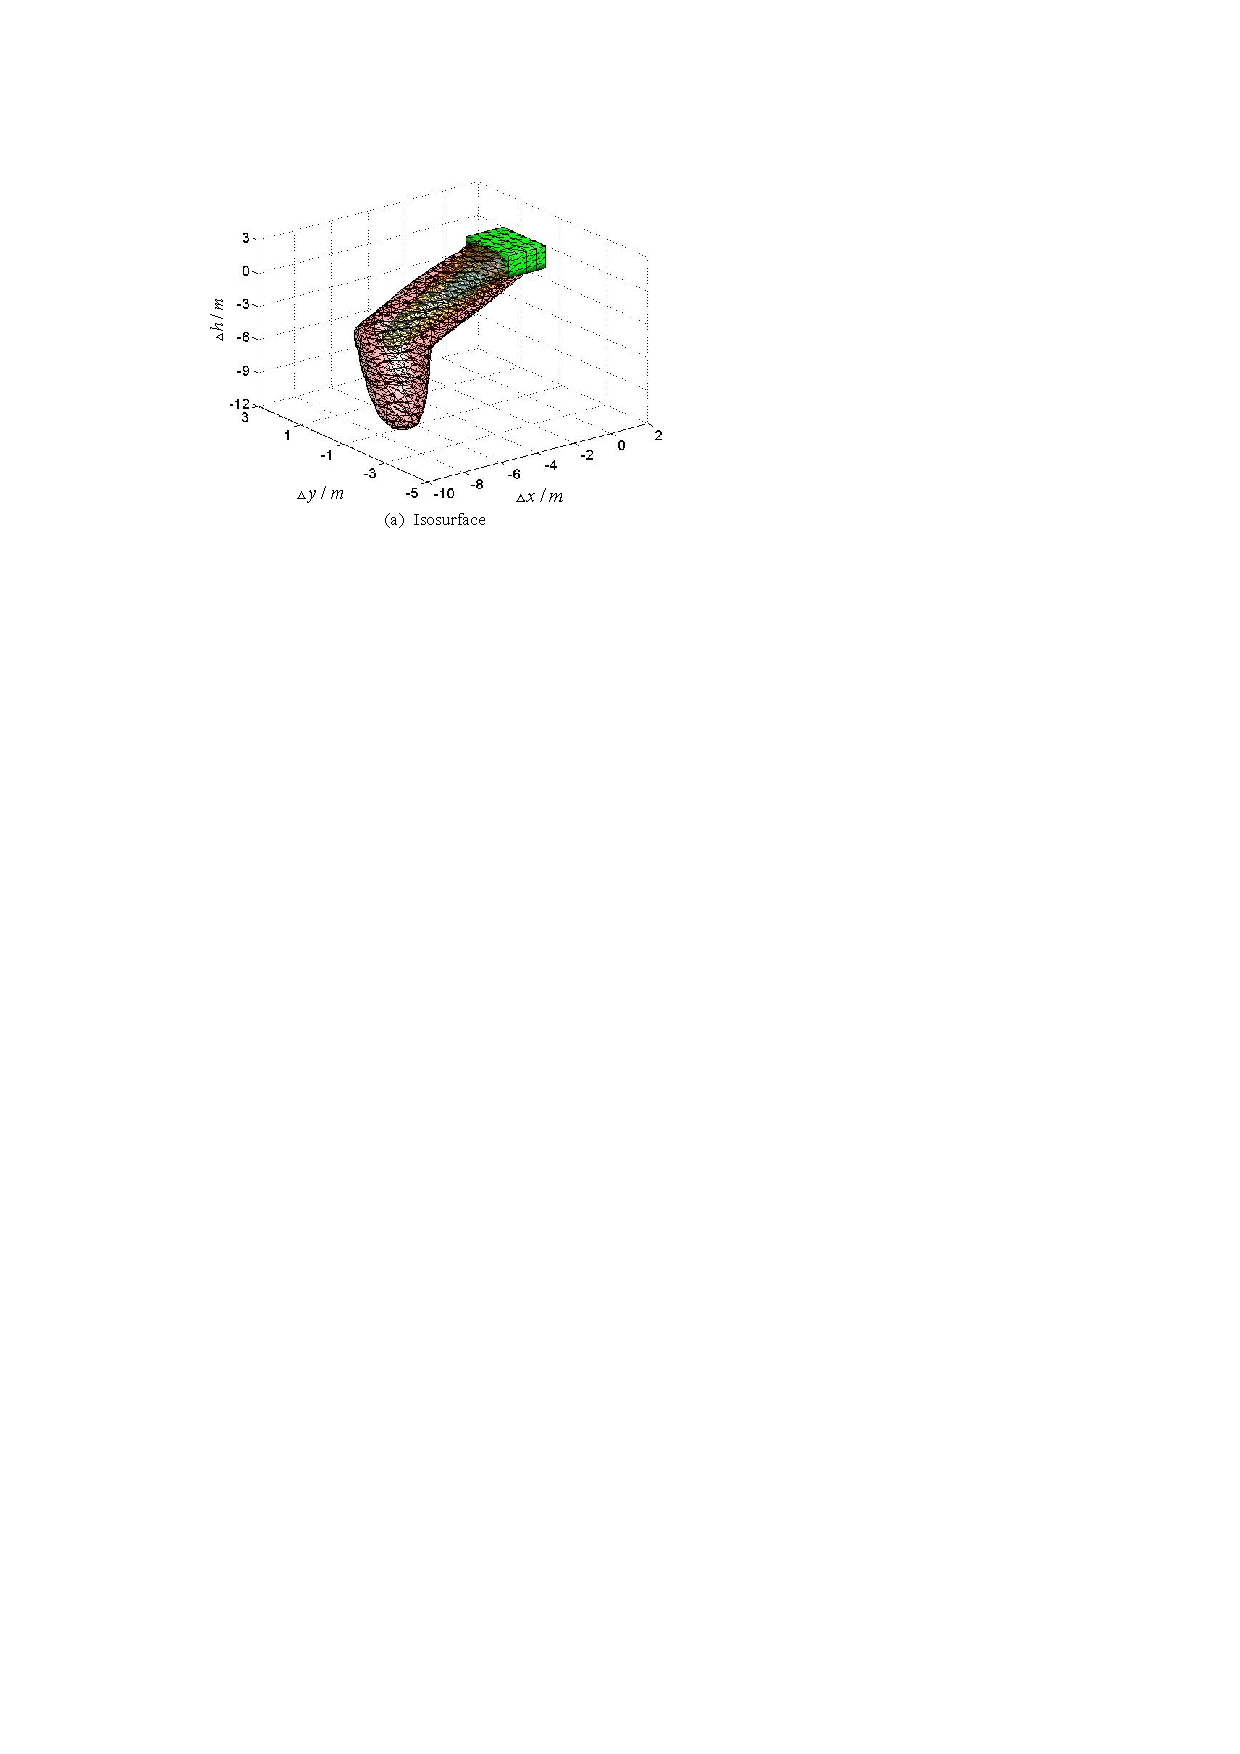
\includegraphics[width=1\linewidth]{Figures/Figs_Ch13/Fig7_1}
	\end{minipage}	\qquad
	\begin{minipage}{0.45\linewidth}
		\centering
		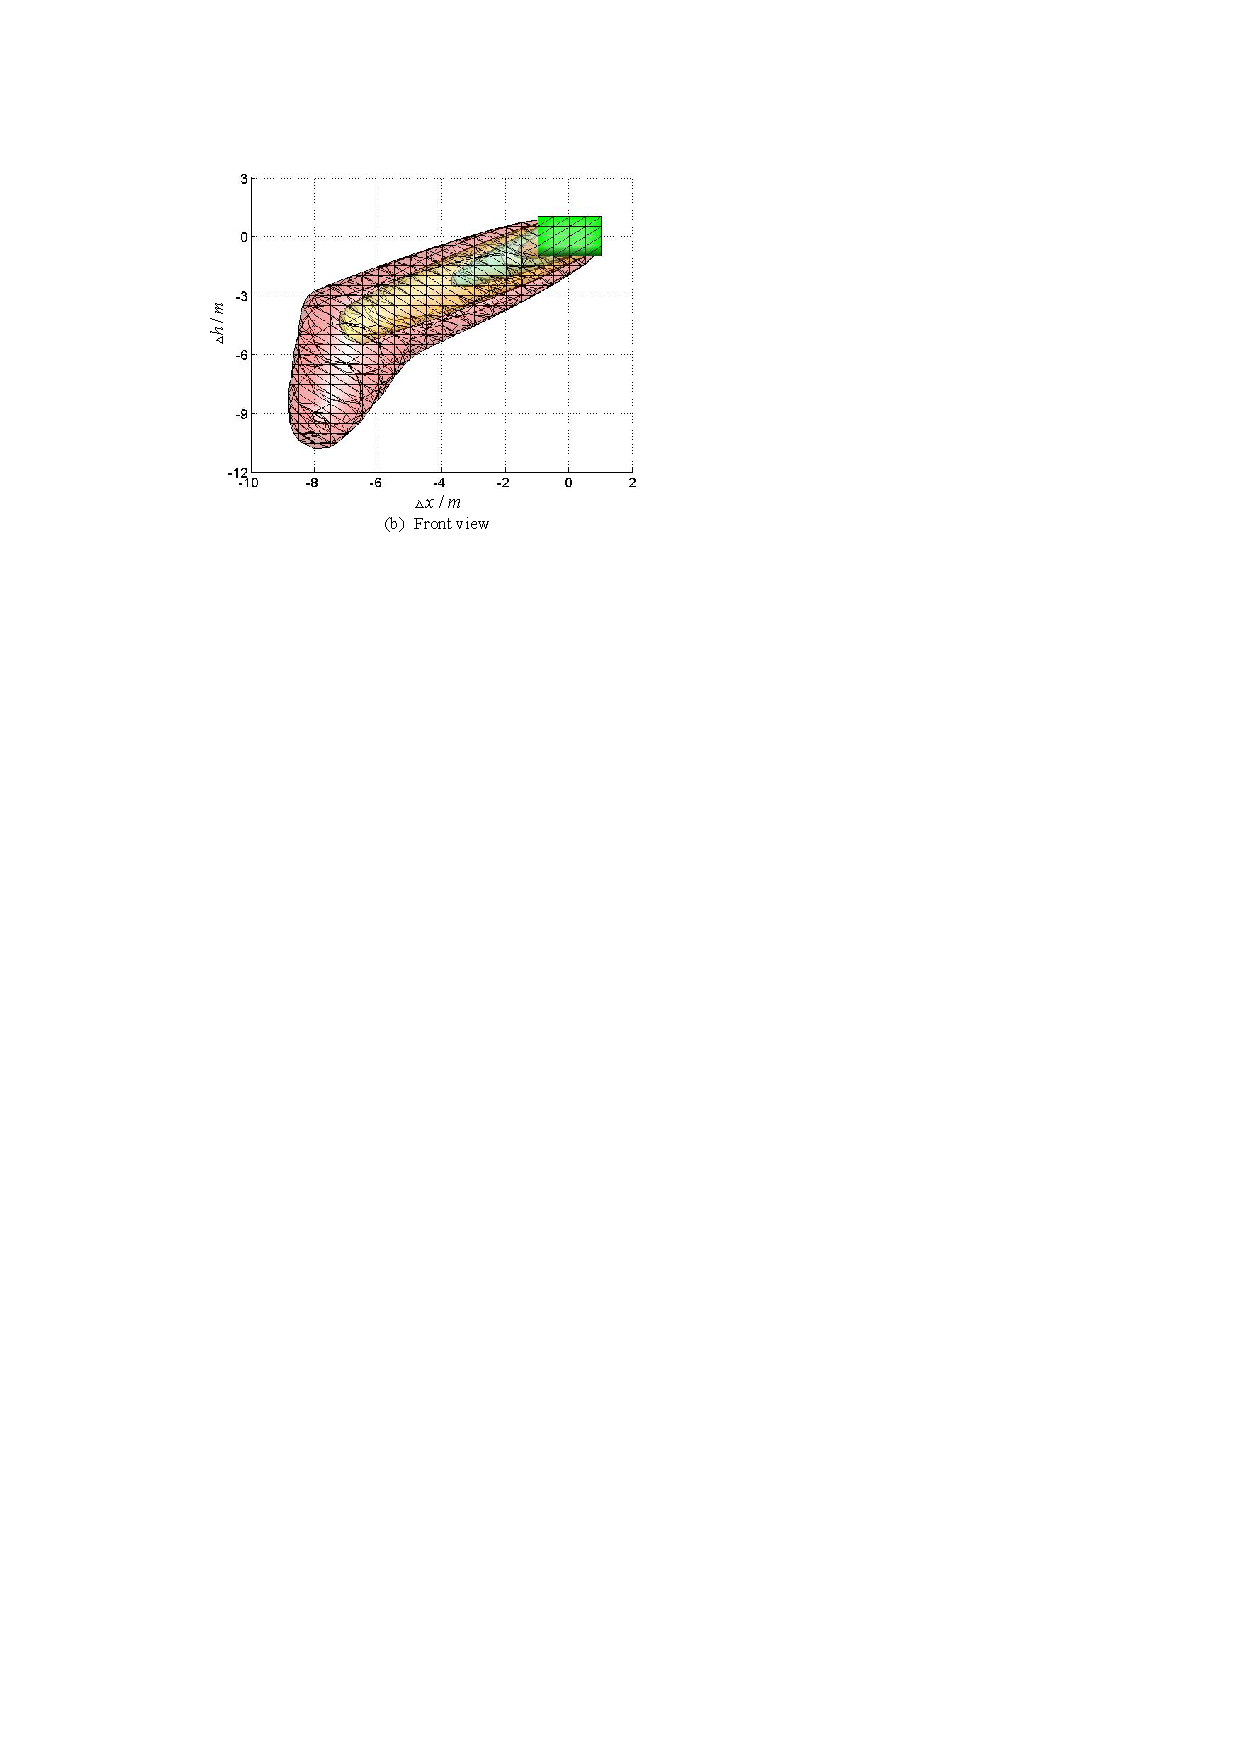
\includegraphics[width=0.9\linewidth]{Figures/Figs_Ch13/Fig7_2}
	\end{minipage}	
	\begin{minipage}{0.45\linewidth}
		\centering
		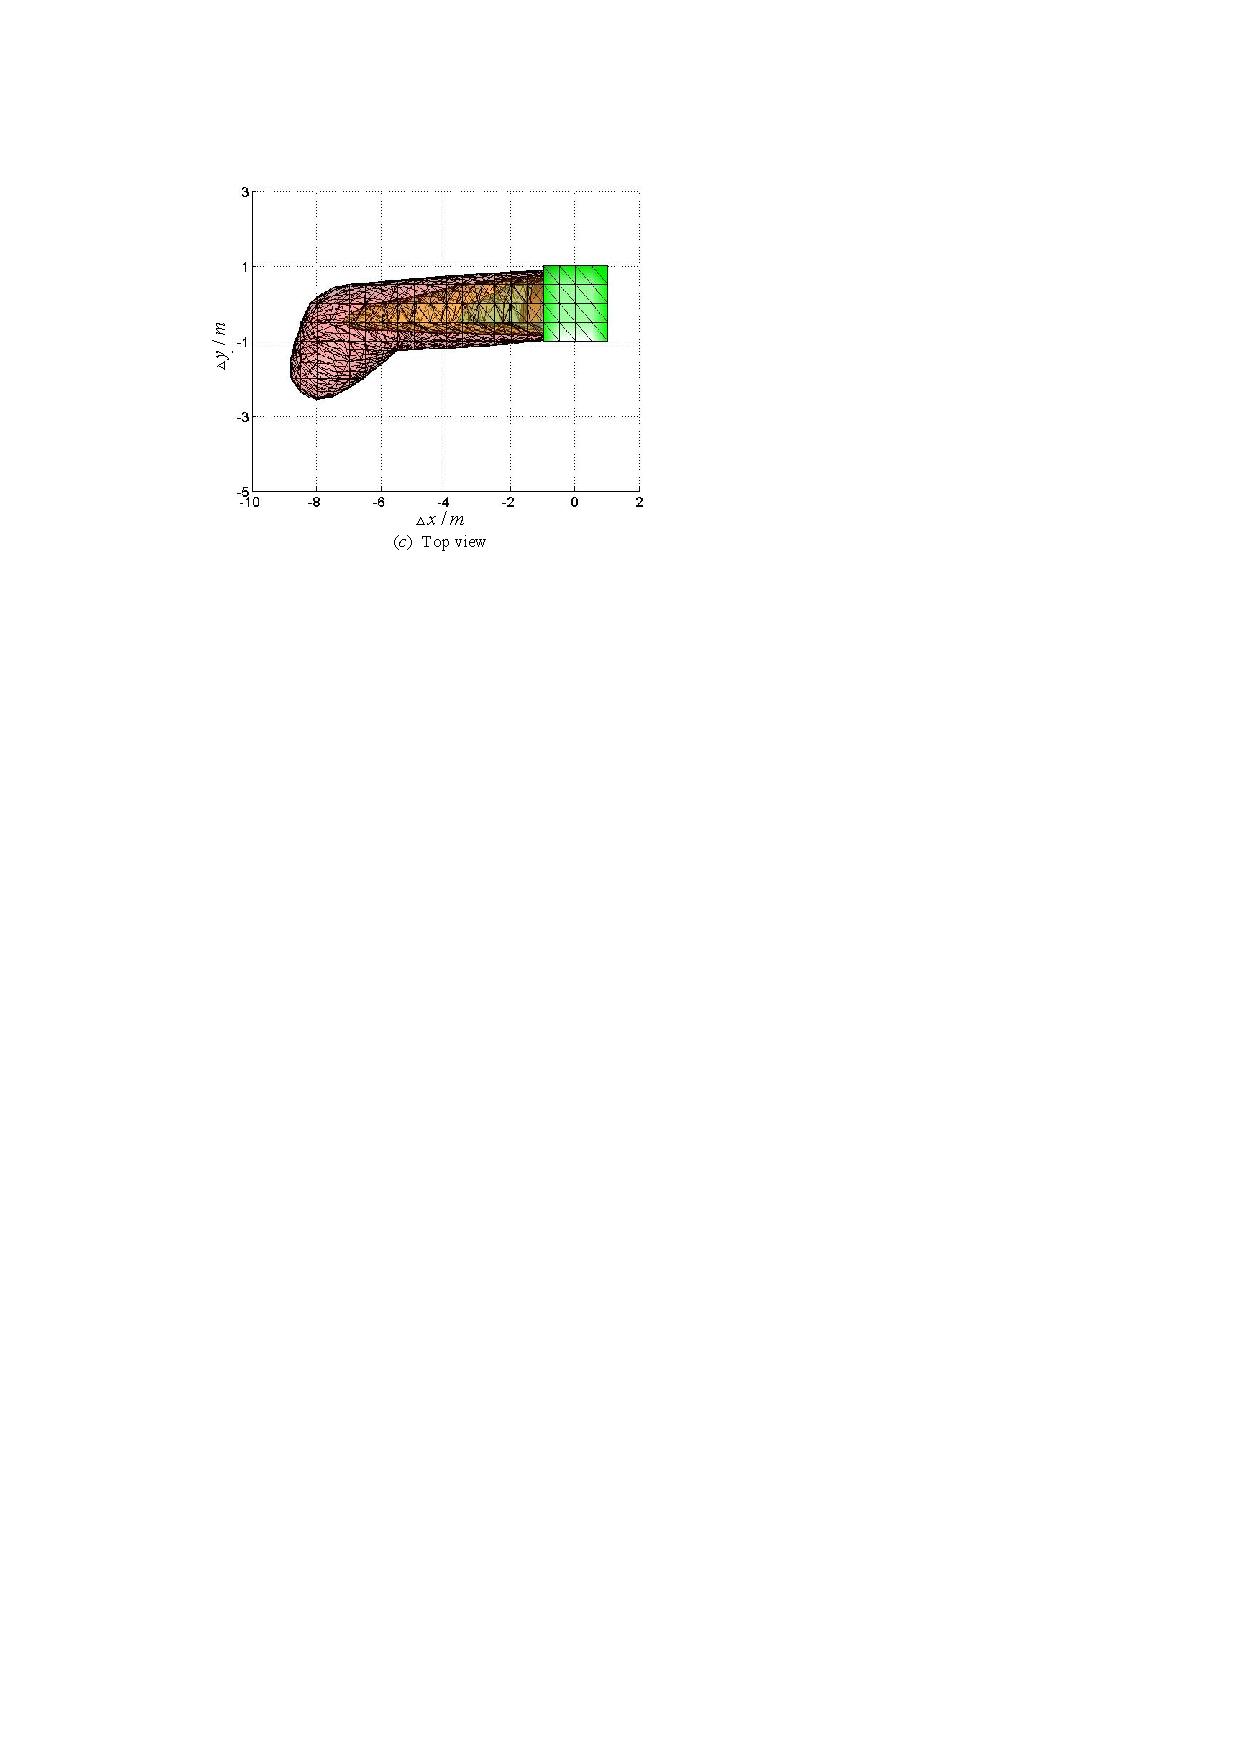
\includegraphics[width=0.9\linewidth]{Figures/Figs_Ch13/Fig7_3}
	\end{minipage}\qquad
	\begin{minipage}{0.45\linewidth}
		\centering
		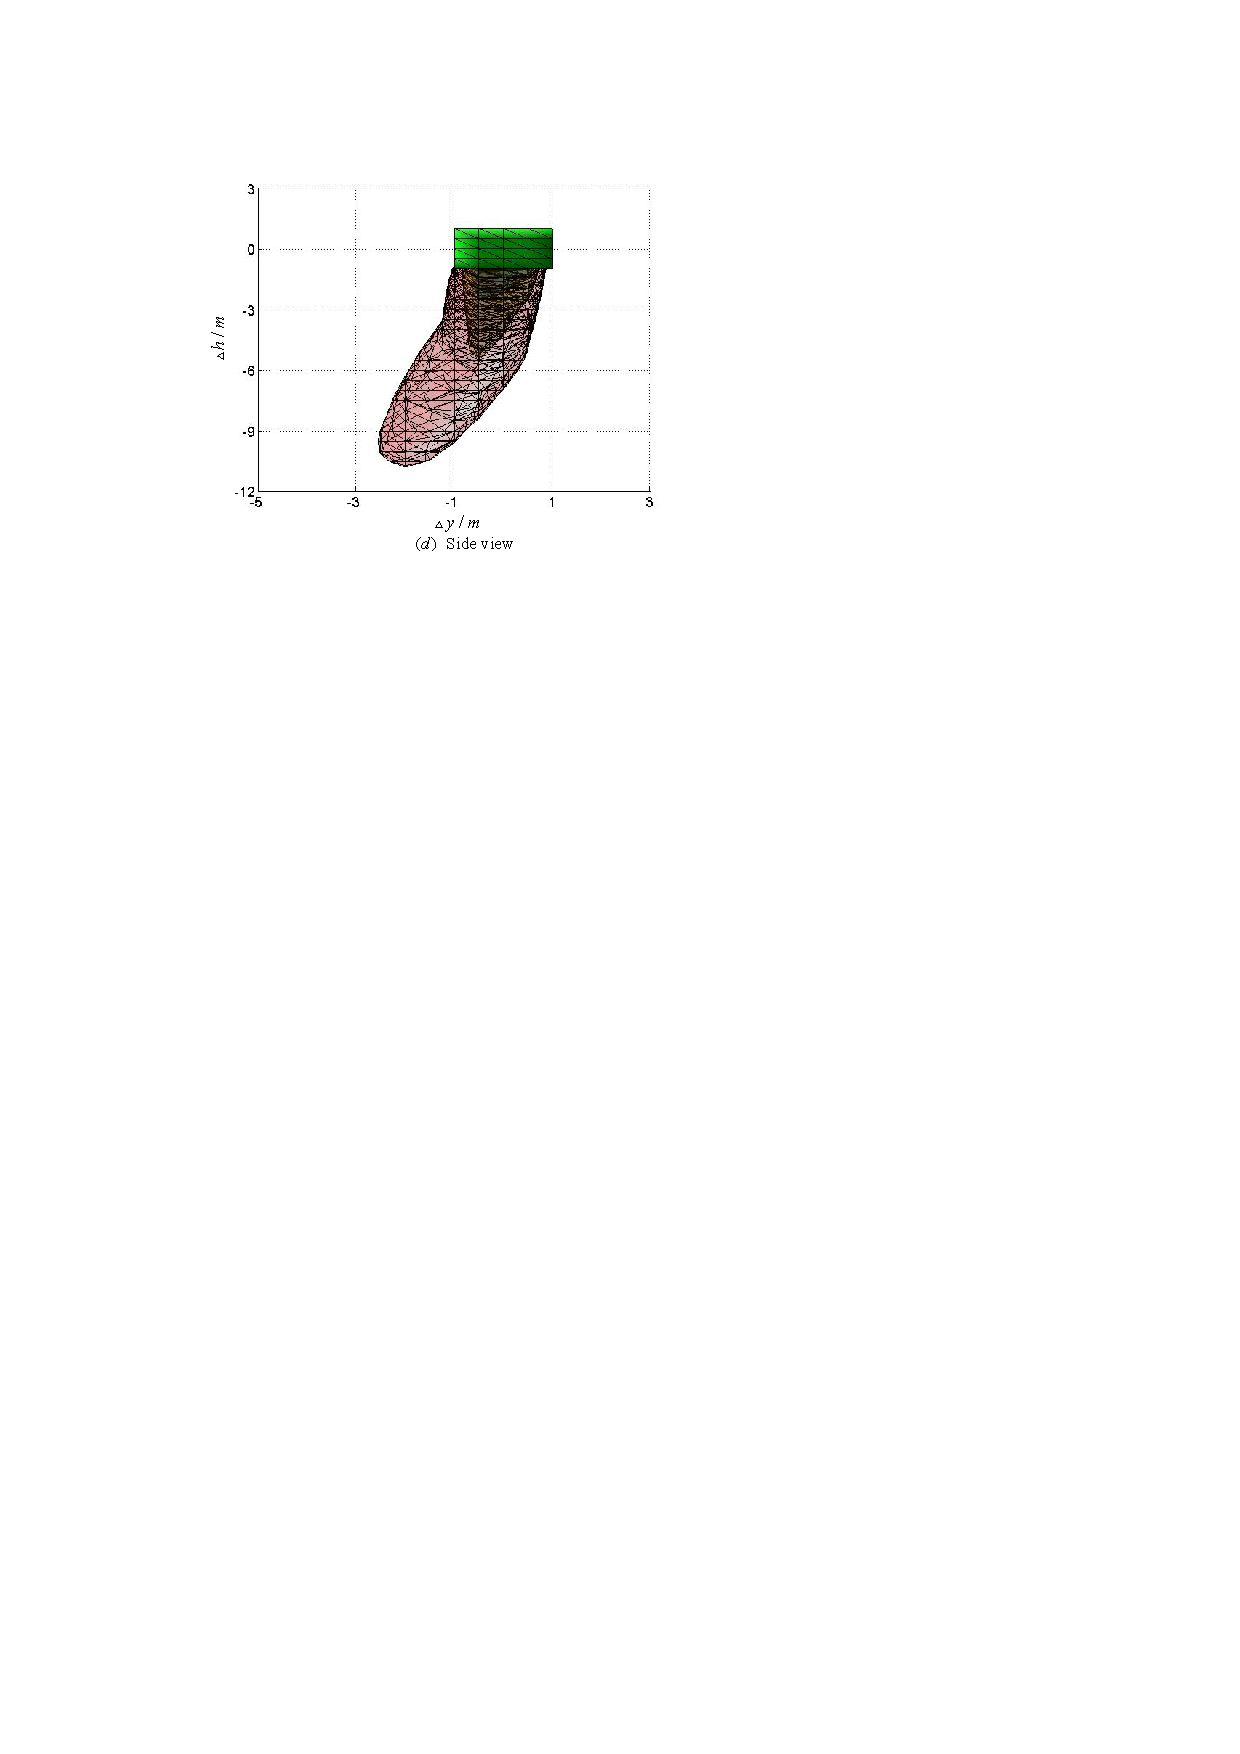
\includegraphics[width=0.9\linewidth]{Figures/Figs_Ch13/Fig7_4}		
	\end{minipage}
	\caption{Isosurface and the corresponding front view of the probability of docking success without considering the wind field.}
	\label{Fig7}
\end{figure}

\subsection{Verification of the results}
In this section, the Monte Carlo method\cite{mackay1998introduction} is used to verify the correctness of the results which are obtained in Sec. \ref{4.2}. The grid points are randomly selected in the state space $ {\cal L} $, where the probability of docking success has been obtained using the stochastic approximation method, and the probabilities of docking success of these grid points are calculated by Monte Carlo method again. Later, the correlation coefficient is adopted to evaluate the relevance of the probabilities of docking success which are obtained by the two methods. The correlation coefficient is computed by
\begin{equation}
\begin{aligned}
r = \frac{{\mathop {\mathop \sum \limits_{j = 1} }\limits^N \left( {{P_j} - \bar P} \right)\mathop {\mathop \sum \limits_{j = 1} }\limits^N \left( {{P_{MC,j}} - {{\bar P}_{MC,j}}} \right)}}{{\sqrt {\mathop {\mathop \sum \limits_{j = 1} }\limits^N {{\left( {{P_j} - \bar P} \right)}^2}\mathop {\mathop \sum \limits_{j = 1} }\limits^N {{\left( {{P_{MC,j}} - {{\bar P}_{MC,j}}} \right)}^2}} }}
\label{eq20}
\end{aligned}
\end{equation}
where $ N $ represents the number of the chosen grid points, $ {P_j}$ and $ {P_{MC,j}} $ represent the probabilities of docking success which are obtained by the stochastic approximation method and Monte Carlo method, respectively. The value  $ {P_{MC,j}} $ is expressed as $ {P_{MC,j}} = {{{n_{{P_{MC,j}}}}} \mathord{\left/{\vphantom {{{n_{{P_{MC,j}}}}} m}} \right.
		\kern-\nulldelimiterspace} m} $, where $ {n_{{P_{MC,j}}}} $ represents the number of the state getting into the target set within the horizon time $ t \in \left[ {0,{t_f}} \right] $ and $ m $ denotes the testing number for the grid point $ {q_j} $. The $ {\bar P} $ and $ {\bar P_{MC,j}} $ represent the average probability and can be denoted by $ \bar P = {{\mathop {\mathop \sum \limits_{j = 1} }\limits^N {P_j}} \mathord{\left/
		{\vphantom {{\mathop {\mathop \sum \limits_{j = 1} }\limits^N {P_j}} N}} \right.
		\kern-\nulldelimiterspace} N}$  and $ {\bar P_{MC,j}} = {{\mathop {\mathop \sum \limits_{j = 1} }\limits^N {P_{MC,j}}} \mathord{\left/
		{\vphantom {{\mathop {\mathop \sum \limits_{j = 1} }\limits^N {P_{MC,j}}} N}} \right.
		\kern-\nulldelimiterspace} N}$ .

\begin{figure}[h]
	\centering
	\begin{minipage}{0.45\linewidth}
		\centering
		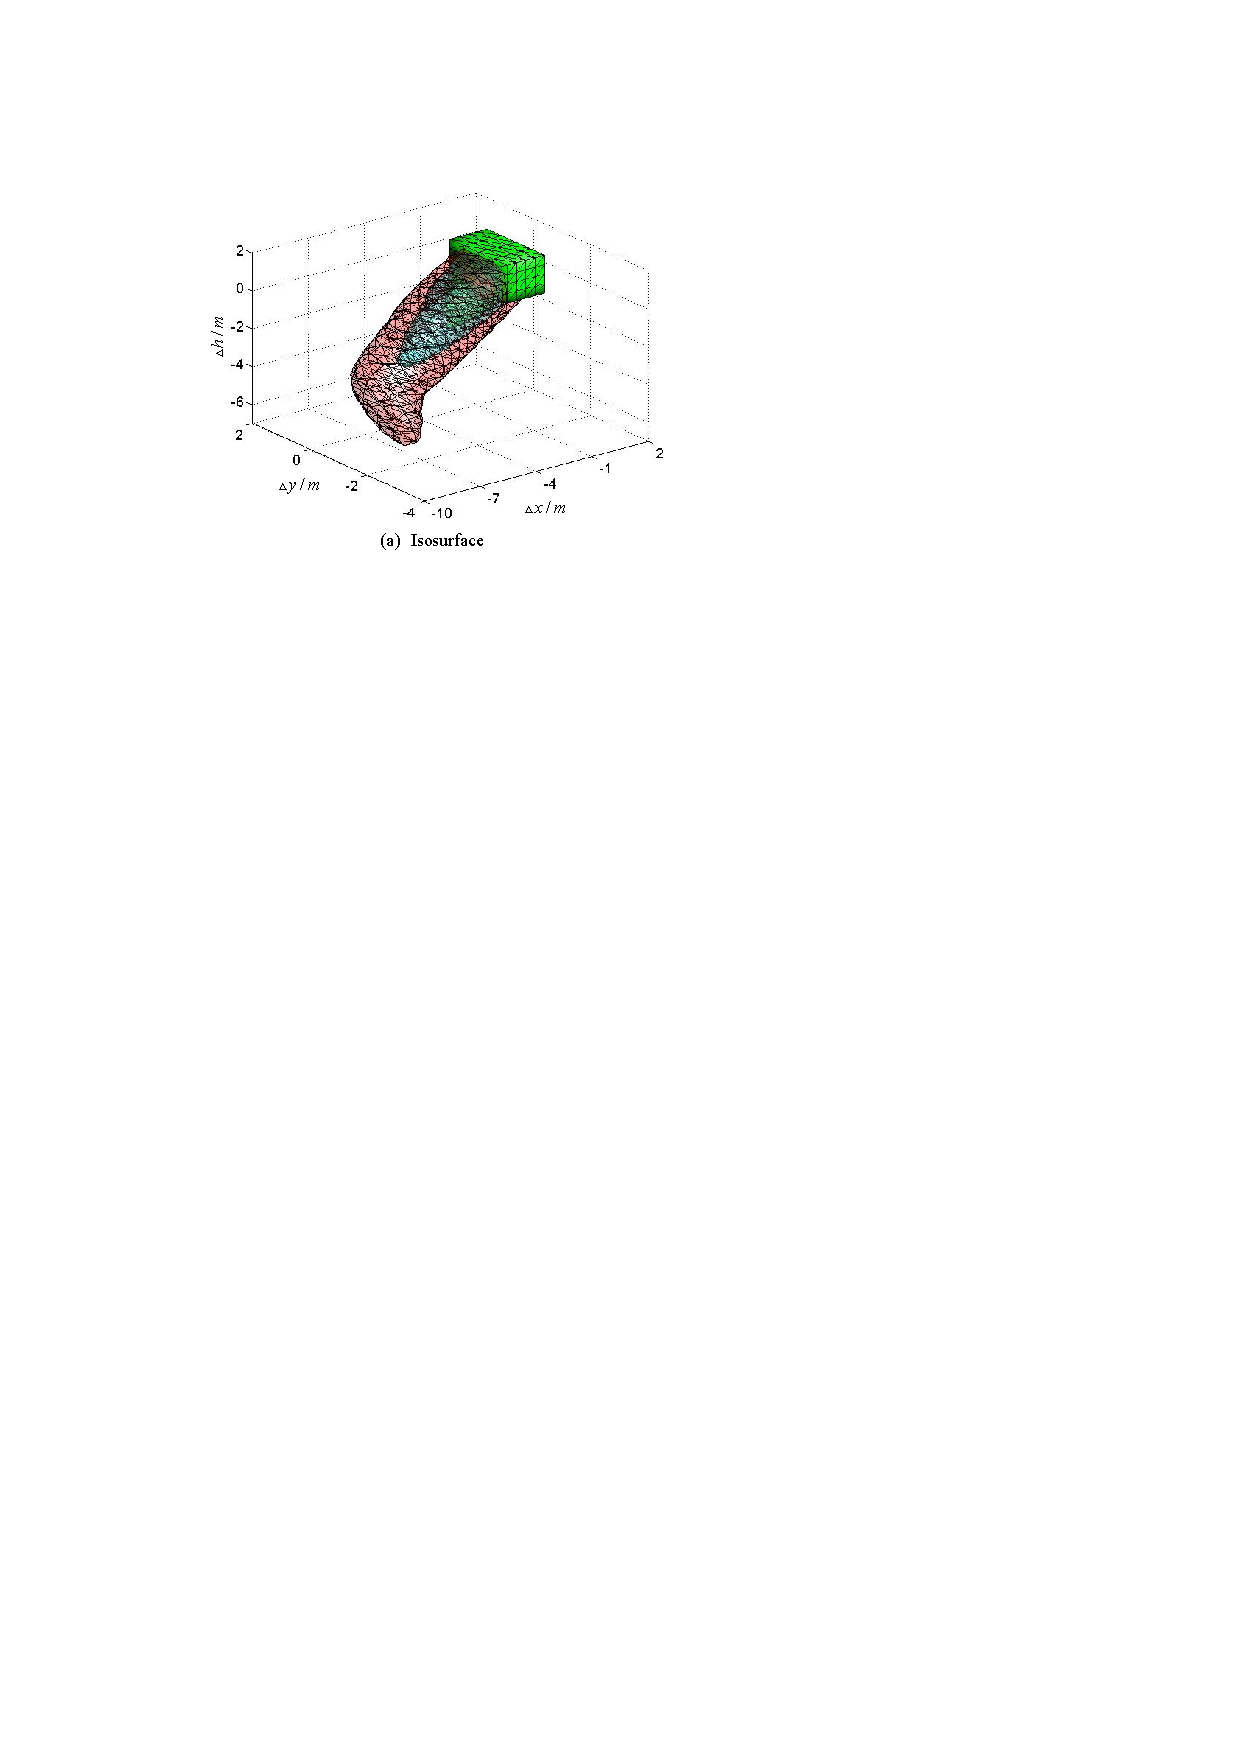
\includegraphics[width=1\linewidth]{Figures/Figs_Ch13/Fig8_1}
	\end{minipage}	\qquad
	\begin{minipage}{0.45\linewidth}
		\centering
		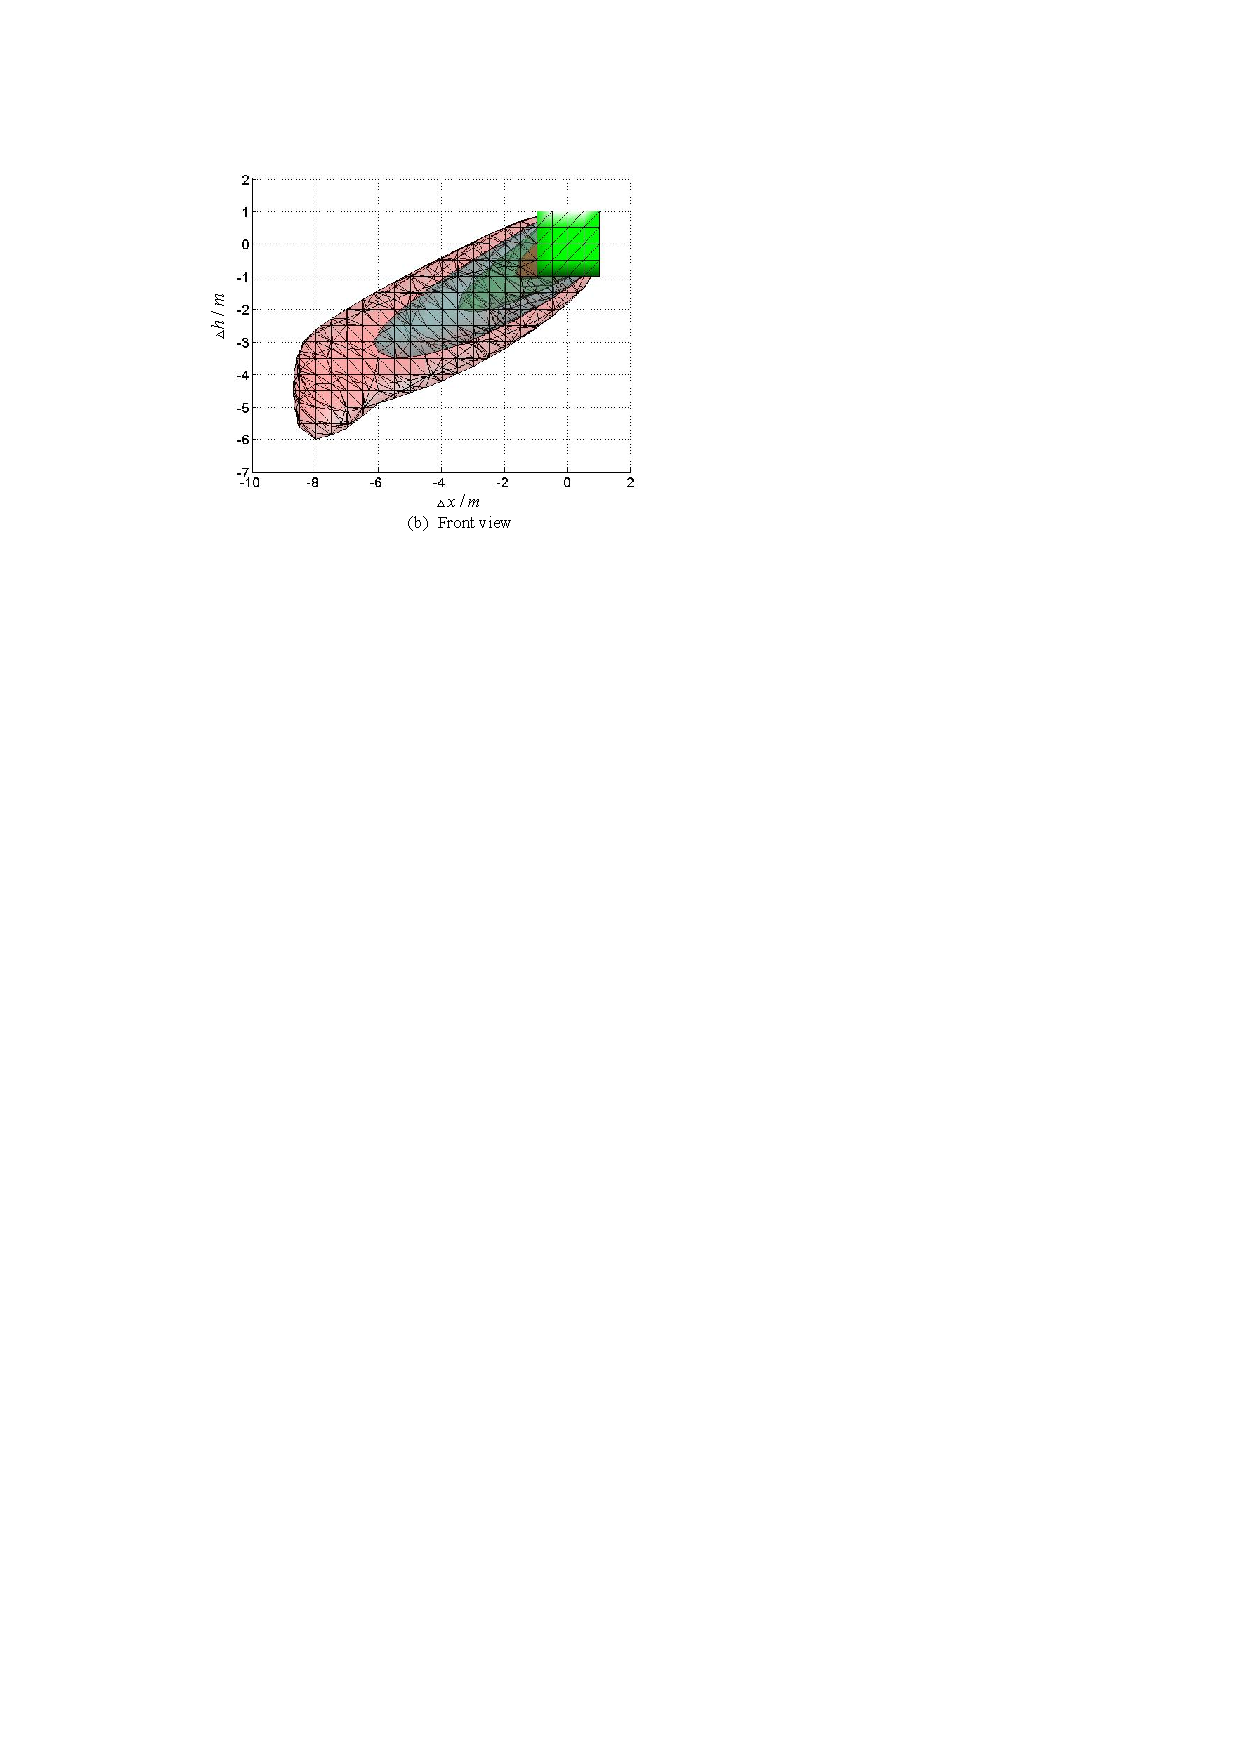
\includegraphics[width=0.9\linewidth]{Figures/Figs_Ch13/Fig8_2}
	\end{minipage}	
	\begin{minipage}{0.45\linewidth}
		\centering
		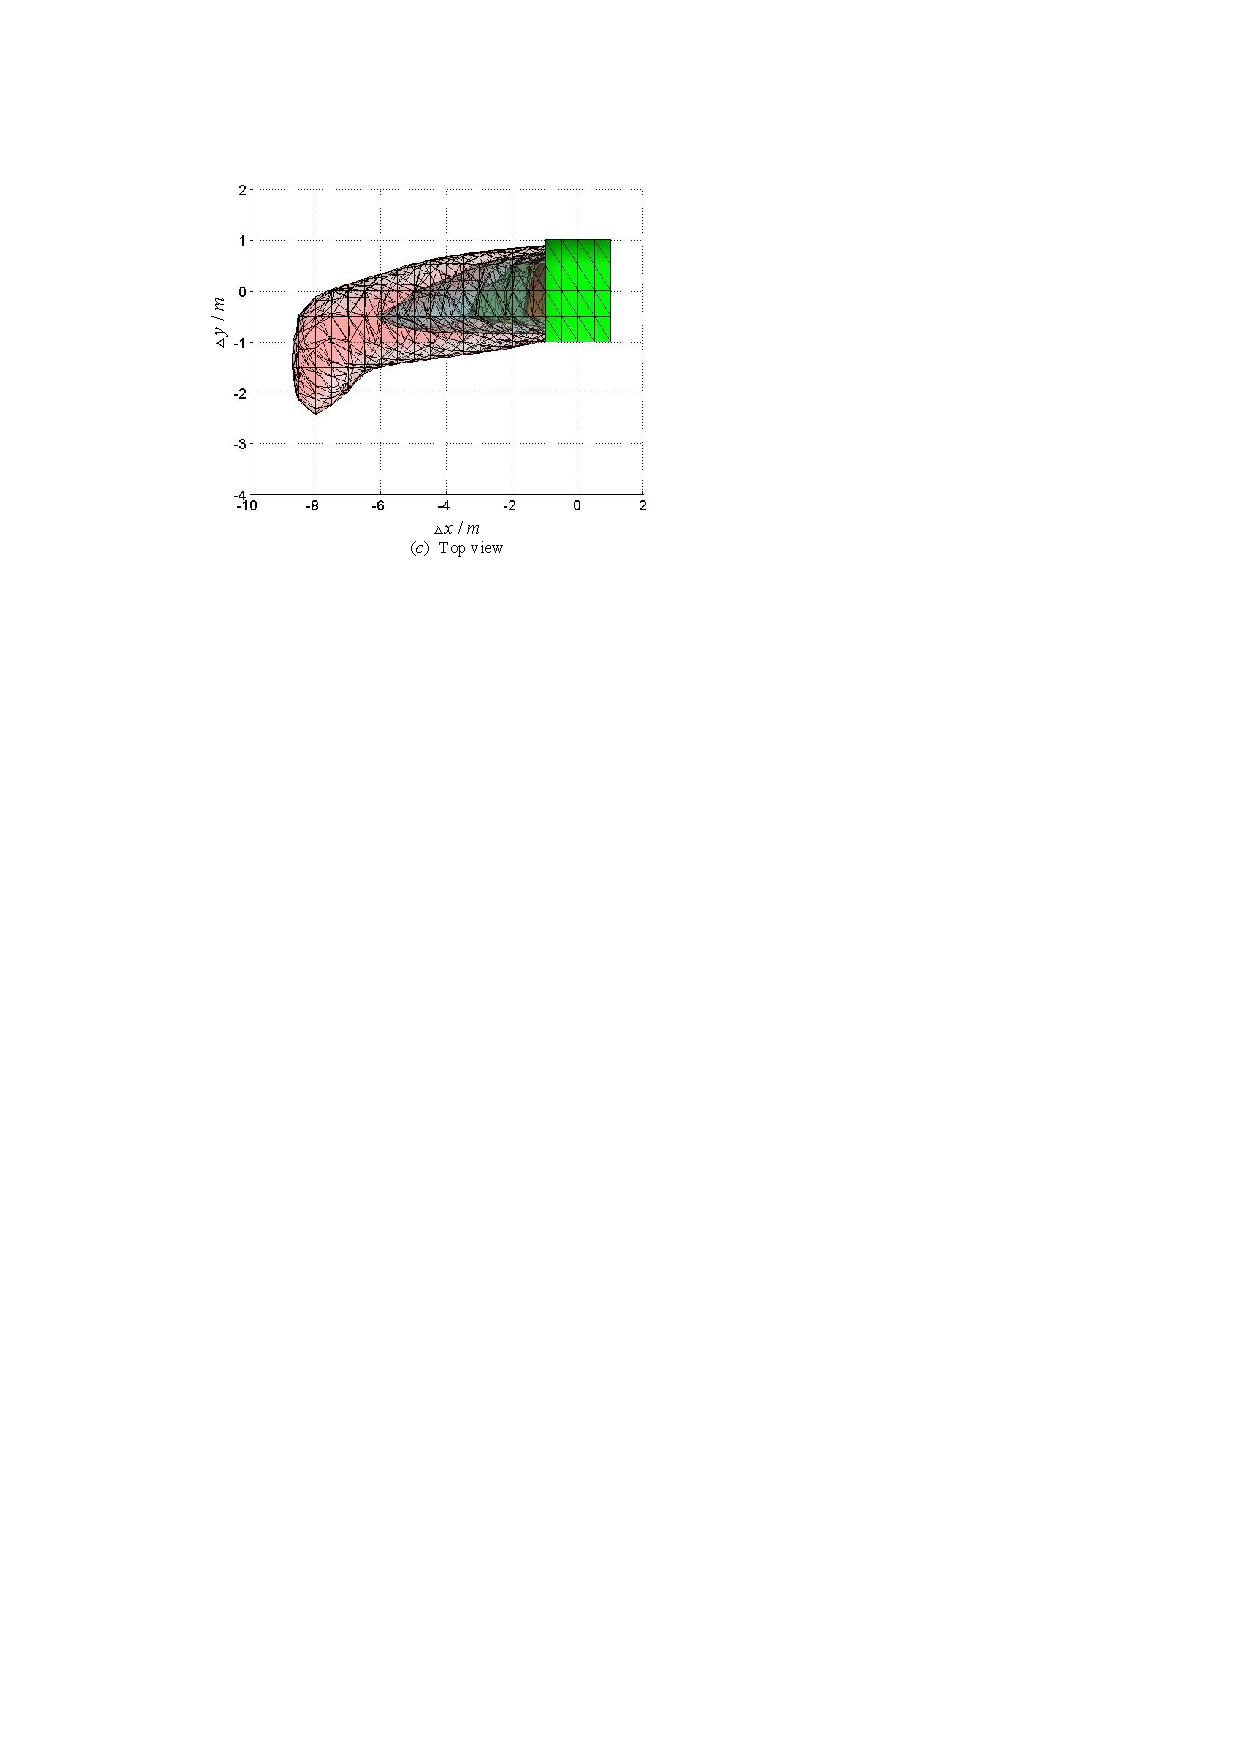
\includegraphics[width=0.9\linewidth]{Figures/Figs_Ch13/Fig8_3}
	\end{minipage}\qquad
	\begin{minipage}{0.45\linewidth}
		\centering
		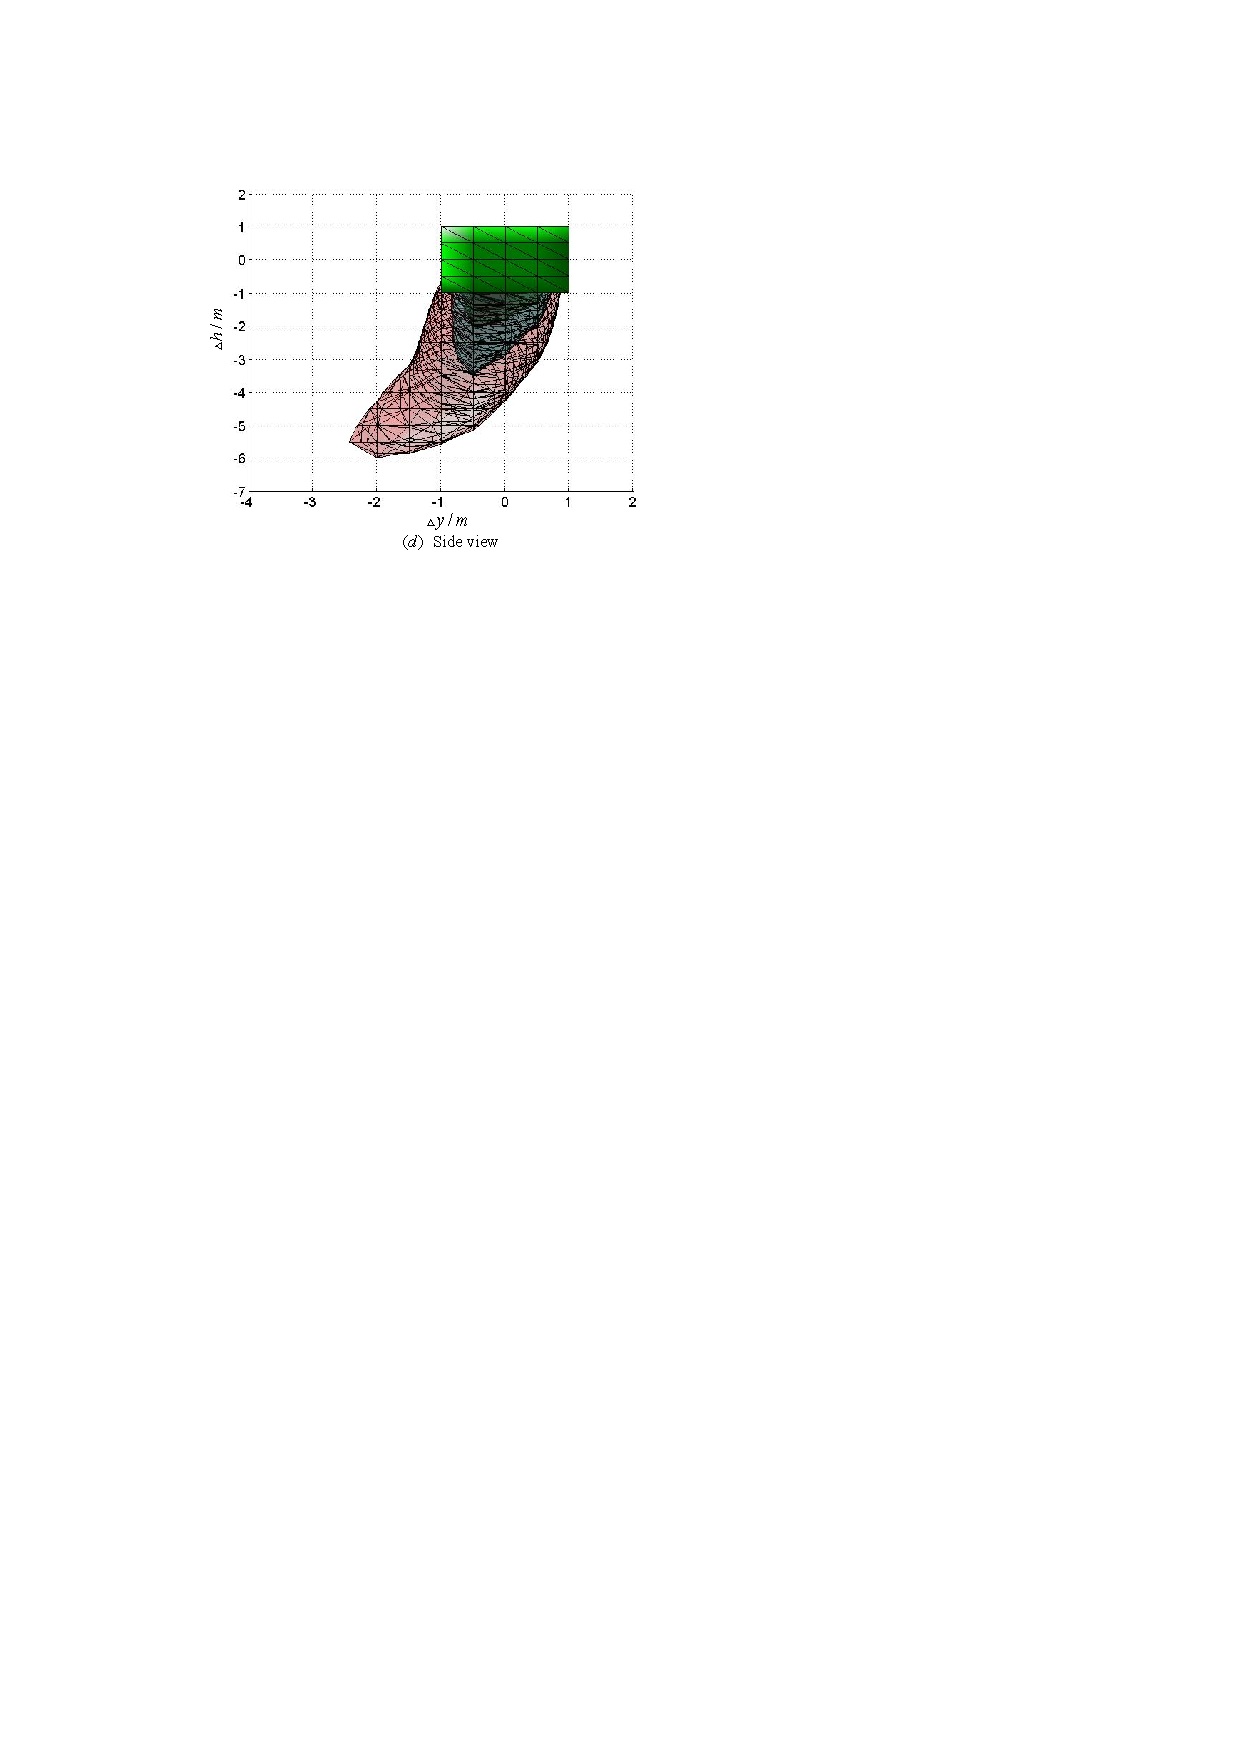
\includegraphics[width=0.9\linewidth]{Figures/Figs_Ch13/Fig8_4}		
	\end{minipage}
	\caption{Isosurface and the corresponding front view of the probability of docking success considering the wind field.}
	\label{Fig8}
\end{figure}

The specific steps of using the Monte Carlo method to get the probabilities of docking success of the grids in state space are as follow:

\textbf{Step 1:} Initialize the state space, target set and the grid points which correspond with that in Sec. \ref{4.1}.

\textbf{Step 2:} Select $ N = 1000 $ grid points randomly in the state space, where the probability of docking success has been obtained using the stochastic approximation method. The selected grid points are denoted as $ {q_j},{\kern 1pt} j = 1, \cdots ,1000$. For each grid point, $ {P_j} $ is known and the testing number is set to be $ m=100 $.

\textbf{Step 3:} The state corresponding to the grid points $ {q_j} $ is taken as the initial state of Eq. (\ref{eq7}). The function $\mathbf  W\left( t \right)$ in Eq. (\ref{eq7}) is a standard 3D Brownian motion, and the mean value and the covariance of $\text d \mathbf W\left( t \right) $  are set to be 0 and $ \sqrt {\Delta t}  $, respectively. By Eq. (\ref{eq8}), whether the corresponding state of ${q_j} $ gets into the target set within the time horizon $ t \in \left[ {0,{t_f}} \right]$ can be determined. If ${q_j} $ can get into the target set, then $ {n_{{P_{MC,j}}}} = {n_{{P_{MC,j}}}} + 1 $.

\textbf{Step 4:} Substitute the results obtained in the above step into Eq. (\ref{eq20}) to obtain the correlation coefficient.

The result shows that the correlation coefficient is 0.96 for $t \in \left[ {0,1} \right] $ and 0.91 for  $t \in \left[ {0,2} \right] $. Therefore, the correctness of the stochastic approximation method to obtain the probability of docking success is demonstrated. Meanwhile, the comparison between the stochastic approximation method and the Monte Carlo method in obtaining the probability of docking success is listed in Table \ref{table4}. The simulation is performed on Matlab R2010a on an ordinary laptop which has a window 7 operating system with a 2.4 GHz processor and 2 GB of RAM. From Table \ref{table4}, it can be observed that the stochastic approximation method is more efficient in calculating the probability of docking success than the Monte Carlo method. The reason for this is that the probability of docking success of each grid point in the state space is calculated directly by the stochastic approximation method. But each grid point in the state space needs to be tested $ m =100 $ to get the probability of docking success using the Monte Carlo method. 
\begin{table}[H]
	\centering
	\caption{The comparison of the simulation times of the two methods.}
	\begin{tabular}{c|c|c}
		\hline
		$ t_f $ & \makecell[c]{Simulation time of\\
			Monte Carlo method}& \makecell[c]{Simulation time of\\
			stochastic approximation method}  \\
		\hline
		1$ s $& 22.70$ \rm{s} $ & 0.22$ \rm{s} $ \\	
		2$ s $ & 38.17$ \rm{s} $ & 0.32$ \rm{s} $  \\
		\hline		
	\end{tabular}
	\label{table4}
\end{table} 
\section{Chapter Summary}
In order to ensure the docking safety in an AR process, a stochastic approximation method is used to obtain the probability of docking success at the docking phase, and the partition of state space probabilistic contour and isosurface can provide decision support for a successful docking.

1) The stochastic differential equation is used in this paper to describe the position of the receiver relative to the tanker, and the wind field and stochastic disturbance are considered in the docking phase.

2) The stochastic approximation method is a kind of model abstract method. By properly choosing the transition probabilities, the solutions of stochastic differential equations are approximated by the discrete-time Markov chain.

3) The probability of docking success of grid points in state space is obtained finally by solving the stochastic differential equations by using the stochastic approximation method.

4) The Monte Carlo method is used to verify the effectiveness of the simulation results. In addition, compared with the Monte Carlo method, the stochastic approximation method can greatly reduce the runtime (See Table \ref{table4}) and thus is more efficient.

In this paper, stochastic differential equations are used to describe the docking phase of aerial refueling, by taking into account wind fields and location-dependent random perturbations. However, in the docking process, since the perturbations situation is complicated, it is a future work to seek a balance between the complicated model and the time consuming to satisfy the real-time estimate for docking success rate.



%\begin{longtable}{|c|c|l|}
%	\caption{\textbf{Nomenclature}} \label{table5} \\
%	\hline
%	\textbf{Symbol} & \textbf{Type} & \textbf{Denotation } \\
%	\hline
%	\endfirsthead
%	\multicolumn{3}{c}{{\tablename\ \thetable{} -- Continued from previous page}} \\
%	\hline
%	\textbf{Symbol} & \textbf{Type} & \textbf{Denotation } \\
%	\hline
%	\endhead
%	\hline \multicolumn{3}{r}{{Continued on next page}} \\
%	\endfoot
%	\hline
%	\endlastfoot
%	$ c_h $ &scalar &  latitudinal correlation coefficient \\\hline
%	$ c_v $ & scalar & longitudinal correlation coefficient \\	\hline
%	$ k $ & scalar & recursive step  \\\hline
%	$ N $ & scalar & the number of the chosen grid points  \\\hline
%	$ p_q^k\left( q \right) $ & scalar & the transition probability from the grid point $ q  $to itself in the $ k $-th step  \\\hline	
%	$ p_{q'}^k\left( q \right) $ & scalar & the probability of transition from the grid point $ q $ to the grid point $ q' $ in the $ k $-th step  \\\hline
%	${P^{\left( k \right)}}\left( q \right) $ & scalar & the probability transited to the grid point $ q $ in the $ k $-th step  \\\hline
%	$ {P_j} $ & scalar & the probabilities of docking success which are obtained by stochastic approximation method  \\\hline
%	$ {P_{MC,j}} $ & scalar & the probabilities of docking success which are obtained by Monte Carlo method  \\\hline
%	$ q $ & scalar & a specific grid point  \\\hline
%	$ r $ & scalar & \makecell [l]{the correlation coefficient of the probabilities of docking success obtained by stochastic \\ approximation  method and Monte Carlo method}  \\\hline
%	$ {t_f} $ & scalar & the end time of the docking phase  \\\hline
%	$ \Delta t $ & scalar & time step  \\\hline
%	$ {V_\text{t}} $ & scalar & tanker speed  \\\hline
%	$ {V_\text{r}} $ & scalar & receiver speed  \\\hline
%	$ \Delta x $ & scalar & the longitudinal distance between receiver and tanker  \\\hline
%	$ \Delta y $ & scalar & the lateral distance between receiver and tanker  \\\hline
%	$ \Delta h $ & scalar & the vertical distance between receiver and tanker  \\\hline
%	${\gamma_\text{r}} $ & scalar & the flight path angle of receiver \\\hline
%	${\varphi_\text{r}} $ & scalar &the azimuth angle of receiver  \\\hline
%	$ \Delta \gamma $ & scalar &the flight path angle of receiver relative to tanker\\\hline
%	$ \Delta \varphi $ & scalar &  the azimuth angle of receiver relative to tanker  \\\hline
%	${\sigma _i}$ & scalar & the element of diagonal matrix 
%	$ \bf{\Gamma }$
%	\\\hline
%	${\bar \sigma} $ & scalar & the max value among  $ {\sigma _i}(i = 1,2,3)$  \\\hline	
%	${\sigma _h}$ & scalar & the variation of lateral stochastic perturbation \\\hline
%	${\sigma _v}$ & scalar & the variation of longitudinal stochastic perturbation\\\hline
%	$ \delta $ & scalar & grid size  \\\hline
%	$\lambda $ & scalar & positive constant related to time step  \\\hline
%	$\eta _i $ & scalar & relative parameter, where $i = 1,2,3$  \\\hline
%	$\cal D $ & set & target set  \\\hline
%	$\cal X $ & set & state constraint set  \\\hline
%	$\cal L $ & set & state space  \\\hline
%	$ Q     $ & set & set of grids \\\hline
%	$ Q_0     $ & set & interior grids of the state space \\\hline
%	$ \partial {Q_{\cal L}}     $ & set & boundary grids of the state space \\\hline
%	$ \partial {Q_{\cal X}}     $ & set & boundary grids of the state constraint set \\\hline
%	$ \partial {Q_{\cal D}}     $ & set & boundary grids of the target set \\\hline
%	$ {{\cal N}_q}     $ & set & adjacent grids of the specific grid point $ q $\\\hline
%	$ {\tilde {\mathbf x}_\text{r/t}}    $ & vector & the position of receiver relative to tanker \\\hline
%	$ \mathbf x_1     $ & vector & the position of the tip of probe \\\hline
%	$ \mathbf y_1    $ & vector & the position of the center of drogue \\\hline
%	$ \alpha \left( {{\mathbf {\tilde x}_\text{r/t}},t} \right)    $ & function & the drift term of the stochastic differential equation \\\hline
%	$ \beta \left( {{\mathbf{\tilde x}_\text{r/t}}} \right)     $ & function & the diffusion term of the stochastic differential equation \\\hline
%	$ {\mathbf a_1}\left( t \right)     $ & function & kinematic equation of the probe \\\hline
%	$ {\mathbf a_2}\left( t \right)     $ & function & kinematic equation of the drogue \\\hline
%	$ {\bf{f}}\left( {{\bf{x}},t} \right)     $ & function & affine transformation in 
%	$ \mathbf x $
%	\\\hline
%	$ \mathbf u\left( t \right)     $ & function & the kinematic states of the tip of the probe with respect to the center of the drogue \\\hline
%	$ \mathbf z\left( t \right)     $ & function & Gaussian process \\\hline
%	$ \rho \left( \mathbf x \right)     $ & function & the spatial correlation function \\\hline
%	$ \mathbf B\left( {{\mathbf x_0},t} \right)     $ & function & standard Brownian motion for a specific position 
%	$ \mathbf x_0 $ \\\hline
%	$ \mathbf B\left( {{\mathbf x},t} \right)     $ & function & stochastic perturbation of current state $ \mathbf x $ \\\hline  
%	$ \mathbf W\left( t \right)      $ & function & a standard 3D Brownian motion \\\hline  
%	$ {\mathbf I_3}     $ & matrix & the 3-by-3identity matrix \\\hline     
%	$ \bf{\Gamma  }   $ & matrix & variance of the random perturbation \\\hline     	
%\end{longtable}



